\documentclass[runningheads,a4paper]{llncs}

\usepackage{url}

%Example for automatically rescaling equations. 
% This is very tricky.
%\begin{equation}
%\label{eq:pimax}
%\resizebox{.55\textwidth}{!}{$
%\begin{split}
%P(\jtable_{2}|\set{E},\ttable) \propto &
%P(\keys = [jack,101],\it{Gr} = A, \it{Sat} = 1|\it{Int} = \class, \it{Rank} = 1, \it{Rat} = 3, \it{Diff}=1)\\
%\times & P(\keys = [jack,102],\it{Gr} = B, \it{Sat} = 2|\it{Int} = \class, \it{Rank} = 1, \it{Rat} = 2, \it{Diff}=2).
%\end{split}$
%}
%\end{equation}

%\usepackage{times}
%\usepackage[normaltitle,normalbib,normalmargins,normalindent]{savetrees}
\usepackage{amsmath}
\usepackage{amsfonts}
\usepackage{amssymb}
\usepackage{graphicx}
\usepackage{url}
%\usepackage{subfigure}
\usepackage{epstopdf}
\setcounter{MaxMatrixCols}{30}
%\usepackage{algorithm}
%\usepackage{algorithmic}
\usepackage{subfigure}
%\usepackage{subcaption}
\usepackage{fancyhdr}
\graphicspath{{../}{figures/}}
\usepackage{todonotes}

\DeclareMathOperator*{\argmax}{argmax}
\DeclareMathOperator*{\argmin}{argmin}
%\DeclareMathOperator{\pattern}{\pi}
\DeclareMathOperator{\Poly}{\mathbf{\mathrm{P}}}
\DeclareMathOperator{\RP}{\mathbf{\mathrm{RP}}}
%\DeclareMathOperator{\FP}{\mathbf{\mathrm{FP}}}
\DeclareMathOperator{\NP}{\mathbf{\mathrm{NP}}}
%\DeclareMathOperator{\E}{\mathbb{E}}
\renewcommand{\d}{\mathbf{d}}

\newcommand{\ZZ}{\mathbf{Z}}

\newcommand{\indep}{\ensuremath{\perp{}\!\!\!\!\!\!\!\perp{}}}
\newcommand{\dep}{\ensuremath{{\perp{}\!\!\!\!\!\!\!\not  \perp{}}}}
%\renewcommand{\L}{\mathcal{L}}
% variables denoting sets of nodes
\newcommand{\V}{V} 
\newcommand{\partC}{\mathcal{C}}
\newcommand{\pattern}{\pi}
% variables denoting nodes
\newcommand{\B}{B}
\renewcommand{\P}{P}
\newcommand{\R}{R}
\newcommand{\X}{X}
\newcommand{\Y}{Y}
\newcommand{\Z}{Z}
\newcommand{\F}{F}
\newcommand{\U}{U}
\newcommand{\W}{W}
\renewcommand{\S}{S}
\newcommand{\C}{C}
\newtheorem{mydef}{Proposition}
%variables for values
%\newcommand{\u}{u}
\renewcommand{\a}{a}
\renewcommand{\b}{b}
\newcommand{\z}{z}
\renewcommand{\v}{v}
\newcommand{\x}{x}
\newcommand{\y}{y}
\newcommand{\p}{p}
\newcommand{\s}{s}
\newcommand{\w}{w} % weights


%statistics
\newcommand{\divergence}{\it{D}}
\newcommand{\score}{\it{score}}
\newcommand{\confidence}{\it{conf}}
\newcommand{\support}{\it{support}}
\newcommand{\loglikelihood}{\it{LOG}}
\newcommand{\lof}{\it{LOF}}
\newcommand{\llmetric}{-L}
\newcommand{\lr}{\it{LR}}
\newcommand{\kl}{\it{KL}}
\newcommand{\el}{\it{EL}}
\newcommand{\mi}{\it{MI}}
\renewcommand{\mid}{\it{ELD}}
\newcommand{\jid}{\it{JID}}
\newcommand{\roc}{\it{ROC}}
\newcommand{\outrank}{\it{OutRank}}
\newcommand{\knn}{\it{KNNOutlier}}
\newcommand{\auc}{\it{AUC}}
\newcommand{\eld}{\it{ELD}}
\newcommand{\fd}{\it{FD}}
\newcommand{\parameter}{\theta}
\newcommand{\parameters}{\bs{\parameter}}
\newcommand{\bic}{\mathit{BIC}}
%random variables and graphical models
% number of values in the domain of a random variable
% variables for BNs
\newcommand{\domvals}{k}
\newcommand{\nodevalue}{\v}
\newcommand{\parvalue}{\mathbf{\pi}} % a single assignment of values to a set of 
%parents
\newcommand{\parvals}{l} % number of values of parent state.
\renewcommand{\r}{r} % CP-table row
\newcommand{\nbhd}{{\mathsf {nbdh}}}
\newcommand{\child}{\mathit{child}}
\newcommand{\parent}{\mathit{pa}}
\newcommand{\parents}{\mathbf{pa}}
\newcommand{\Parents}{\mathbf{PA}}
\newcommand{\family}{F} % families, family formulas
\newcommand{\vpi}{\mathbf{pa}} % for vectors of variable assignments
\renewcommand{\l}{\ell} % class label
\newcommand{\states}{r} % number of states of a variable
%\newcommand{\value}{value}
\newcommand{\mb}{\set{mb}} % markov blanket of a variable, vector-valued
\newcommand{\ssize}{N} % number of rows in join table; size of sample
\newcommand{\mbstates}{m} % number of states in Markov blanket
\newcommand{\frequency}{fr}
\newcommand{\pseudo}{\ast}
\newcommand{\counts}{+}
\newcommand{\weighted}{\ast}
\newcommand{\halpern}{H}
\newcommand{\Thetaa}{\theta}
\newcommand{\instance}{I}

%logic notation
%\newcommand{\predicate}{\phi}
\newcommand{\functor}{f}
\newcommand{\outdomain}{V}
\newcommand{\indomain}{\Omega}
\newcommand{\variable}{X} % first-order variable
\newcommand{\population}{\mathcal{P}}
\newcommand{\entity}{x}
\newcommand{\formula}{\phi}
\newcommand{\formulas}{\mathcal{\phi}}
\newcommand{\literal}{l}
\newcommand{\conjunction}{\set{C}} % conjunction of literals
\newcommand{\fterm}{\f} % open function term
\newcommand{\fterms}{F} % set of function terms, also nodes in JBN
\newcommand{\term}{\sigma}
\newcommand{\Terms}{\bs{\sigma}}
\newcommand{\constant}{a}
\newcommand{\constants}{\bs{\constant}}
\newcommand{\gterm}{g} % ground term
\newcommand{\gterms}{\bs{\gterm}} %list of ground terms
\newcommand{\vterm}{x} % variable term
\newcommand{\vterms}{\bs{\vterm}} % list of variable terms
\newcommand{\assign}{A} % assignment of values to Bayes net
\newcommand{\resultset}{\mathbb{R}}
\newcommand{\grounds}{\#}
\newcommand{\grounding}{\gamma}
\newcommand{\groundall}{\Gamma}
\newcommand{\vars}{\mathit{Var}} % variables in a conjunction
\newcommand{\igraph}{I} % instance-level dependency graph.
\newcommand{\assignment}{\set{a}}
\newcommand{\atom}{\ell}
\newcommand{\gnode}{\alpha}
\newcommand{\gfamily}{\ground{f}}
\newcommand{\numformulas}{m}
\newcommand{\structure}{\mathcal{S}}
% logic programs
\newcommand{\program}{\mathcal{B}}
\newcommand{\clause}{\mathcal{c}}
\newcommand{\head}{\mathit{head}}
\newcommand{\body}{\mathit{body}}
\newcommand{\crule}{\mathit{cr}} % combining rule
\newcommand{\level}{\mathit{level}} % rank of function symbols in LP

%datbase schema
\newcommand{\rcolumns}{R}
\newcommand{\ecolumns}{E}
\newcommand{\dtable}{T} % can't use \table. Generic database table
\newcommand{\datatable}{D} % generic data table, not necessarily part of database.
\newcommand{\jtable}{J} % join table
\newcommand{\Ejoin}{$J^{+}$}
\newcommand{\jtables}{m}
\newcommand{\rtable}{R} % relationship table
\newcommand{\etable}{E} % entity table.
\newcommand{\ttable}{X} % target table
\newcommand{\nextended}{n}
\newcommand{\row}{r}
\newcommand{\rows}{\mathit{rows}}
\newcommand{\col}{j}
\newcommand{\cols}{\mathit{cols}}
\newcommand{\unary}{\f} % to denote a unary or attribute function
\newcommand{\numatts}{u} % to denote the number of unary or attribute functions.
\newcommand{\g}{g} % alternative for function
\newcommand{\relational}{\mathbf{r}} % denotes a generic relational functors, can be both relationship or descriptive attribute of relationship
\newcommand{\Relation}{R} % denotes a generic boolean relation
% a special type of literal conjunction that assigns a value %to each variable
\providecommand{\keywords}{\textbf{keywords: }}
\newcommand{\loss}{\ell}
\newcommand{\class}{c} % the class attribute
\newcommand{\classlabel}{y} % the class label
\newcommand{\classifier}{\mathcal{M}}
\newcommand{\target}{t} % target object
\newcommand{\Target}{T}
\newcommand*\rfrac[2]{{}^{#1}\!/_{#2}}
\newcommand{\object}{o}
\newcommand{\Class}{C}
\newcommand{\scorediff}{\Delta}
\newcommand{\model}{B}
\newcommand{\modelprob}{\theta}
\newcommand{\profile}{P}
% the probabilities defined by a model, like conditional probabilities in a BN
\newcommand{\Targetcount}{\Gamma}
\newcommand{\neighbor}{n}
\newcommand{\feature}{V} % feature or desc attribute of object or link
\newcommand{\features}{\bs{v}} % features 
\newcommand{\Features}{\bs{V}}
\newcommand{\attribute}{a} % nonclass attribute of target object
\newcommand{\attributes}{\bs{a}}
\newcommand{\rels}{\bs{R}} % chain of relationships.
\newcommand{\maxpath}{\rho}
\newcommand{\eatts}{\it{1Nodes}}
\newcommand{\ratts}{\it{2Nodes}}
\newcommand{\atts}{\it{ANodes}}
\newcommand{\marginalize}{\it{margin}}
%special functions
\newcommand{\AVG}{\it{AVG}}
\newcommand{\instances}{n} % counts number of occurrences in DB
\newcommand{\prob}{p} % frequency of formula true in in DB

%variables denoting graphs or models
\newcommand{\mln}{M}
\newcommand{\G}{G}
\newcommand{\node}{V}
\newcommand{\nodes}{V}
\newcommand{\edges}{E}
\newcommand{\clique}{C}
\newcommand{\cliques}{\mathcal{\clique}}
\newcommand{\cliquevalue}{c}
\newcommand{\graph}{G}
\newcommand{\M}{M}
\newcommand{\J}{J}
\renewcommand{\H}{H}
\newcommand{\K}{K} % component
\renewcommand{\O}{O} % oracle
\renewcommand{\path}{\rho} % path, also foreignkey path
% Markov nets
\newcommand{\potential}{\Psi}
% database schema
\newcommand{\type}{\tau} % to denote a generic type
\newcommand{\E}{E} % for entity tables
\newcommand{\e}{e} % for specific entities
\newcommand{\f}{f}
\newcommand{\new}{\it{new}}
\renewcommand{\c}{c}
\renewcommand{\R}{R} % for relationship tables
\newcommand{\A}{A} % for attributes
\newcommand{\T}{T} % for tables generically
\newcommand{\New}{N}
\newcommand{\D}{\mathcal{D}} % for database instance
\newcommand{\databases}{\set{D}} % the number of databases
\newcommand{\vocab}{\mathcal{\L}} % for logical vocabulary associated with database
\newcommand{\name}{\mathit{name}} % generic attribute
\newcommand{\dom}{\mathit{dom}} % domain of attributes
\newcommand{\etables}{\alpha} % entity tables
\newcommand{\rtables}{\beta} % relationship table number
% specific constructs for examples


\newcommand{\team}{\it{T}}
\newcommand{\player}{\it{P}}
\newcommand{\match}{\it{M}}


\newcommand{\director}{\it{Director}}
\newcommand{\movie}{\it{Movie}}
\newcommand{\user}{\it{User}}
\newcommand{\corr}{\it{\rho}}
\newcommand{\student}{\mathit{Student}}
\newcommand{\I}{\mathit{I}}
\newcommand{\course}{\mathit{Course}}
\newcommand{\prof}{\mathit{Professor}}
\newcommand{\person}{\mathit{Person}}
\newcommand{\TA}{\mathit{TA}}
\newcommand{\actor}{\mathit{Actor}}
\newcommand{\age}{\mathit{age}}
\newcommand{\intelligence}{\mathit{intelligence}}
\newcommand{\diff}{\mathit{difficulty}}
\newcommand{\reg}{\mathit{Registered}}
\newcommand{\win}{\it{win}}
\newcommand{\ra}{\mathit{RA}}
\newcommand{\bt}{\mathit{blood type}}
\newcommand{\grade}{\mathit{grade}}
\newcommand{\gpa}{\mathit{gpa}}
\newcommand{\jack}{\mathit{Jack}}
\newcommand{\jill}{\mathit{Jill}}
\newcommand{\smith}{\mathit{Smith}}
\newcommand{\cmpt}{\mathit{CMPT120}}
\newcommand{\hi}{\mathit{Hi}}
% various constants
\newcommand{\true}{\mathit{T}}
\newcommand{\false}{\mathit{F}}
\newcommand{\normalconstant}{Z} % the normalization constant

% orderings
\newcommand{\pred}{\mathit{pred}}
%procedure names and such
\newcommand{\join}{\textsc{Join-Frequencies}}
\newcommand{\linus}{\textsc{Linus }}
\newcommand{\foil}{\textsc{Foil }}
\newcommand{\MLN}{\textsc{MLN}}
\newcommand{\treetilde}{\textsc{TILDE }}

%%%
%undirected models
\newcommand{\pot}{\phi} % potential function
%\newcommand{\theHalgorithm}{\arabic{algorithm}}
\newcommand{\test}{test}
\def\set#1{\mathbf{#1}}
\def\bs#1{\boldsymbol{#1}}
\def\ground#1{\overline{#1}}


\renewcommand{\Qconj}{\Appendterm{\FG{\TT} = \TV} {\QC}} % Use TT instead of \Ground{TI} (TI notation not defined in this paper)

\usepackage{graphicx} 

% Sep 7: mention that David Poole et al. use logistic regression too.
% Another view of the random regression result: if I use proportion/frequency as an aggregation function to produce an aggregate feature for propositionalization, then propositionalization is equivalent to the geometric mean as a combining rule.
% To fix the likelihood non-result about likelihood maximization, see email to Ted. Should also fix the inconsistency/incoherence problem.

\renewcommand{\marginpar}[1]{\fixneeded{(AS MARGINPAR) #1}}

\newcommand{\fixneeded}[1]{\textbf{[\footnotesize #1]}}

% Force text to appear on a separate line from a subsection header
\newcommand{\forcesubsectext}{\hskip 1pt\vskip 0pt\noindent}

% Lists in running text
% We'll probably want to regularize these later
\newcommand{\point}[1]{\noindent\emph{#1}.}
\newcommand{\subpoint}[1]{#1:}
\newcommand{\keypoint}[1]{{\em #1}}
\newcommand{\strongpoint}[1]{\paragraph{#1.}}

\newcommand{\iid}{i.i.d.}
\newcommand{\etal}{\textit{et al.}}

\graphicspath{{../../}{figures/}}

\title{Fast Learning of Relational Dependency Networks}

\author{Oliver Schulte, Zhensong Qian, Arthur E. Kirkpatrick\\ Xiaoqian Yin, Yan Sun 
%\thanks {This research was supported by a Discovery Grant to Oliver Schulte from the Canadian Natural Sciences and Engineering Council. And Zhensong Qian was also supported by a grant from the China Scholarship Council.}
}
\authorrunning{  Oliver Schulte, Zhensong Qian, Arthur E. Kirkpatrick et al.}
\institute{ School of Computing Science, Simon Fraser University, Canada\\
\{oschulte,zqian,ted,xiaoqian\_yin,sunyans\}@sfu.ca\\}
             

\date{\today}
\begin{document}

\maketitle



\begin{abstract} 
A Relational Dependency Network (RDN) is a directed graphical model widely used for multi-relational data. These networks allow cyclic dependencies, necessary to represent relational autocorrelations. We describe an approach for learning both the RDN's structure and its parameters, given an input relational database: First learn a Bayesian network (BN), then transform the Bayesian network to an RDN. Thus fast Bayes net learning translates into fast RDN learning. The BN-to-RDN transform comprises a simple, local adjustment of the Bayes net structure and a closed-form transform of the Bayes net parameters. This method can learn an RDN for a dataset with a million tuples in minutes. We empirically compare our approach to state-of-the art RDN learning methods that use functional gradient boosting, on five benchmark datasets. Learning RDNs via BNs scales much better to large datasets than learning RDNs with boosting, and provides competitive accuracy in predictions.\end{abstract}


\section{Introduction} \label{sec:intro} Learning graphical models is one of the main approaches to extending machine learning for relational data. 
Dependency networks (DNs) \cite{Heckerman2000} are one of the major classes of graphical generative models, together with Markov networks and Bayesian networks (BNs) \cite{Pearl1988}. We describe a new approach to learning dependency networks: first learn a Bayesian network, then convert the Bayesian network to a dependency network. 
This hybrid approach combines the advantages of learning with Bayesian networks and performing inference with relational dependency networks. 
Our experiments show that the hybrid learning algorithm can produce dependency networks for large complex databases, with up to one million records, and up to 19 predicates. The predictive accuracy of the learned dependency networks is competitive with those constructed by state-of-the-art function gradient boosting methods.
% It scored higher on the conditional log-likelihood metric on all five benchmark datasets. On the Area Under Curve metric Bayesian network learning scored better on 2/5, worse on 2/5. 
Bayesian network learning scales substantially better   to larger datasets than the boosting methods.
%
Our main contributions are:
\begin{enumerate}
\item A faster approach for learning relational dependency networks: first learn a Bayesian network, then convert it to a dependency network.
\item A closed-form log-linear discriminative model for computing the relational dependency network parameters from Bayesian network structure and parameters.
\item Necessary and sufficient conditions for the consistency of the learned relational dependency network. Consistency refers to the existence of a single joint probability distribution that induces the various conditional probability distributions defined by the dependency network \cite{Heckerman2000}.
\end{enumerate}
  
 \section{Relational Dependency Networks and Bayesian Networks} We review the definition of dependency networks and their advantages for modelling relational data. We assume familiarity with the basic concepts of Bayesian networks \cite{Pearl1988}.
 
 \subsection{Dependency networks and Bayesian networks} Like Bayesian networks, the structure of a dependency network is defined by a graph whose nodes are random variables and whose edges are directed. Unlike Bayesian networks, a dependency network graph may contain cycles and bi-directed edges. As with Bayesian networks, the parameters of dependency networks are conditional distributions over the value of a child node given its parents. The difference lies in the characteristic independence property of dependency networks: each node is independent of {\em all} other nodes given an assignment of values to its parents, which is generally not the case for Bayesian networks.
In graphical model terms, the parents of a node in a dependency network form a {\em Markov blanket}: A minimal set of nodes such that assigning them values will make this node independent of the rest of the network. 

Consequently, a parameter in a dependency network effectively specifies the probability of a node value given an assignment of values to all other nodes. 
%Such conditional probabilities play an important role in statistical inference, for example in the widely used Gibbs sampling procedure \cite{Lunn2000}. 
We therefore refer to such conditional probabilities as \defterm{Gibbs conditional probabilities}, or simply Gibbs probabilities.\footnote{In the terminology of dependency networks \cite{Heckerman2000},  Gibbs  probabilities are referred to as local probability distributions.}
% The WinBUGS system refers to them as full conditional probabilities~\cite{Lunn2000}.}. 
Gibbs sampling can be used to derive a joint distribution from the Gibbs probability DN parameters \cite{Heckerman2000,Neville2007}. This is the counterpart to the Bayes net product formula that derives a joint distribution from the network's conditional probability parameters. 

\begin{figure}[htbp]
\begin{center}
%\resizebox{0.78\textwidth}{!}{
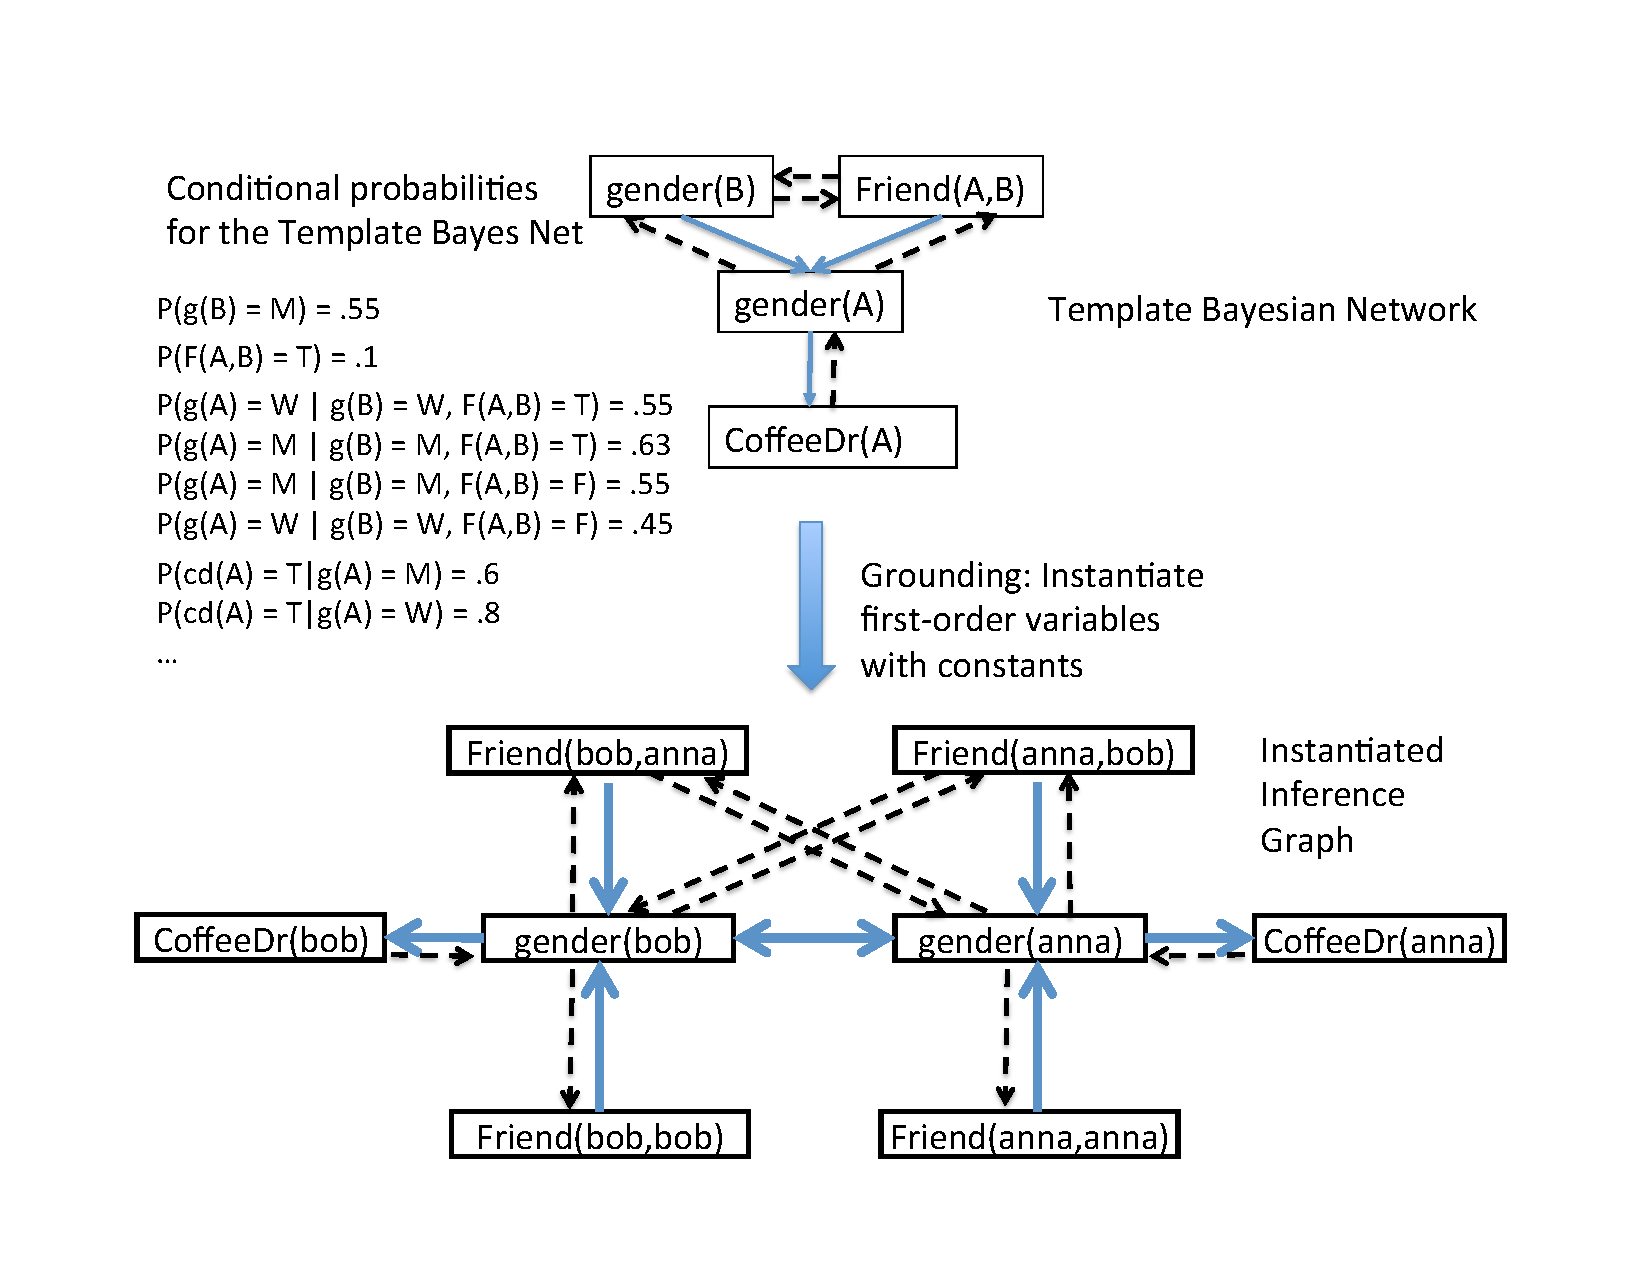
\includegraphics[width = 0.7 \textwidth]{figures/dn}
%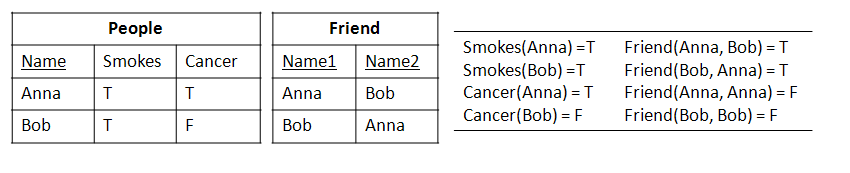
\includegraphics[width=1\textwidth]{database.png}
%}
\caption{A Bayesian/dependency template network (top) and the instantiated inference graphs (bottom). Edges derived from the BN template are shown as blue and solid. Edges added by the BN-to-DN transformation are shown as black and dashed. Thus the edge set in the DN comprises both solid and dashed arrows. Notice that instantiating the BN induces a bi-directed edge between $\it{gender}(bob)$ and $\it{gender}(anna)$. \label{fig:dn}
We use uppercase for predicates (Boolean functors) and lowercase for other functors.}
\end{center}
\end{figure}

 
\subsection{Relational Dependency Networks} There are various different notational systems for defining random variables in relational structures, of equivalent expressive power. We adopt function-based notation from logic  for graphical-relational models \cite{Russell2010,Poole2003}. A functor is a function or predicate symbol. Each functor has a set of values (constants) called the \textbf{domain} of the functor. In this paper we consider only functors with finite domains. A \textbf{Parametrized Random Variable} (PRV) is of the form $f(\term_{1},\ldots,\term_{k})$ where $\functor$ is a functor 
and each $\term_{i}$ is a first-order variable or a constant.
 %or a constant denoting an individual. 
 A Parametrized Bayesian Network structure is a directed acyclic graph whose nodes are PRVs. A \textbf{relational dependency network structure} (RDN) is a directed graph whose nodes are PRVs.
RDNs extend dependency networks for relational data by using knowledge-based model construction \cite{Neville2007}:
%
%\fixneeded{Oliver, my phrasing is likely wrong. My goal is to start this section with how RDNs extend DNs. How does that work?} 
%
 The first-order variables in a template RDN graph are instantiated for a specific domain of individuals to produce an {\em  instantiated} or {\em ground} propositional DN graph, the \defterm{inference graph}. Figure~\ref{fig:dn} gives a dependency network template and its  inference graph. Given an edge in the template RDN, instantiating both the parent and the child of the edge with the same grounding produces an edge in the inference graph. An example Gibbs probability distribution for the inference graph (abbreviating functors to their first letter) is
$$P(\it{g(anna)}|\it{g(bob)}, \it{CD(anna)}, \it{F(anna,bob)},\it{F(bob,anna)},\it{F(anna,anna)}).$$

\noindent Both the structure and the parameter space of RDN models offer special advantages for relational data \cite{Neville2007,Natarajan2012}: 

\begin{enumerate}
\item Dependency network structures are well-adapted for relational data because they allow cyclic dependencies, so grounding a dependency network template is guaranteed to produce a valid dependency network.
%
%\fixneeded{Is there anything about the next paragraph that limits it to RDNs or does it all apply to DNs? If it applies to DNs, let's move it to DN section above.}
\item Relational prediction  requires aggregating information from different linked individuals \cite{Natarajan2008}. 
%Two common approaches are combining rules \cite{Kersting2007} and aggregation functions \cite{Getoor2007c}. 
In a dependency network parameter, the aggregation encompasses the entire Markov blanket of a target node, whereas for Bayesian network parameters, the aggregation encompasses only its parents.
\end{enumerate}
%
%One of the challenges for inference on relational data is that, unlike the non-relational \iid{} case, {\em a single template node may be instantiated into multiple predictors} \cite{Natarajan2008}. In the inference graph of Figure~\ref{fig:dn}, each gender of a friend of $\it{anna}$ adds one relevant predictor for the value of $\it{gender}(anna)$. The number of predictors is therefore not fixed by the model, but depends on the number of individuals related to the target individual. Relational prediction therefore requires aggregating information from different linked individuals. Two common approaches are (i) combining rules \cite{Kersting2007} and (ii) aggregation functions \cite{Getoor2007c}. In a dependency network, the aggregation encompasses the entire Markov blanket of a target node, whereas in a Bayesian network, the aggregation encompasses only its parents.
%\fixneeded{Check if we still need this after full editing.}

\section{Learning Relational Dependency Networks via Bayesian Networks}
Our algorithm for rapidly learning relational dependency networks
begins with any relational learning algorithm for Bayesian networks. We then apply a simple, fast transformation of the resulting Bayesian network to a relational dependency template. Finally we apply a closed-form computation to derive the dependency network parameters from the Bayesian structure and parameters. Figure~\ref{fig:bn-flow} shows the program flow. 
%for computing a Gibbs probability using the log-linear equation.

\paragraph{BN-to-DN structure conversion.}
Converting a Bayesian network structure to a dependency network structure is simple: for each node, add an edge pointing to the node from each member of its BN Markov blanket~\cite{Heckerman2000}.  The result contains  bidirectional links between each node, its children, and its co-parents (nodes that share a child with this one). 
%
%This simply means adding edges into the node from each of its children and bidirectional links between the node and its co-parents (nodes that share a child with this one). 
This is equivalent to the standard moralization  method for converting a BN to an undirected model \cite{Domingos2009}, except that the dependency network contains bi-directed edges instead of undirected edges. Bidirected edges have the advantage that they permit  assignment of different parameters to each direction, whereas undirected edges have only one parameter.
 
\begin{figure}[t]

\begin{center}
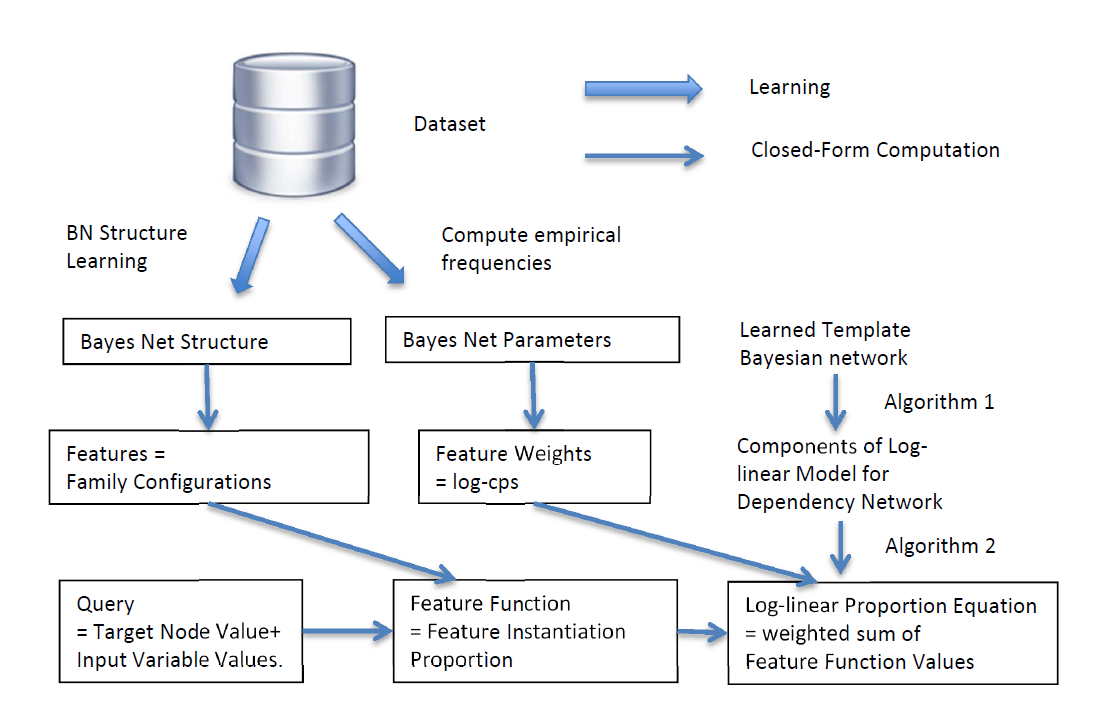
\includegraphics[width=0.7\textwidth]{bn-regress.png}
\caption{The program flow for computing Gibbs probabilities from a template Bayesian network. Features and weights are computed from the Bayes net. Feature function values are computed for each query. \label{fig:bn-flow}}
\end{center}

\end{figure}

\paragraph{BN-to-DN parameter conversion.} Converting Bayesian network parameters to dependency network parameters is simple for propositional \iid{} data: solve for the Gibbs conditional probabilities given Bayesian network parameters. The propositional result is as follows. A \defterm{family} comprises a node and its parents. A \defterm{family configuration} specifies a value for a child node and each of its parents. For example in the Bayesian network of Figure~\ref{fig:dn}, a family configuration is 
$$\it{gender}(\A) = \Man, \it{Friend}(\A,\B) = \true, \it{gender}(\B) = \Man.$$
For propositional data, an assignment of values to the Markov blanket of a target node assigns a unique configuration for each family whose child is the target node or one of its children. Hence the Markov blanket induces a {\em unique} log-conditional probability for each such family configuration. The probability of a target node value given an assignment of values to the Markov blanket is then proportional to {\em the exponentiated sum of these log-conditional probabilites} \cite[Ch.14.5.2]{Russell2010}. 

With relational data, different family configurations such as the one above can be simultaneously instantiated, {\em multiple times.}  We adapt the propositional log-linear equation for relational data by replacing the unique log-conditional probability with the {\em expected} log-conditional probability that results from selecting an instantiation of the family configuration uniformly at random. The probability of a target node value given an assignment of values to the Markov blanket is then proportional to the exponentiated sum of the expected log-conditional probabilites. %Without this normalization, features with more instantiations carry exponentially more weight. 
We describe the resulting closed-form equation in the next section.




\begin{algorithm}[htbp]
%\linesnumbered
\SetKwData{Calls}{Calls}
\SetKwData{Notation}{Notation}
%\begin{algorithmic}
%{\footnotesize
%\STATE {\em Input}: Database $\D$ with $\etable_1,..\etable_e$ entity tables, functors $\F$, variable number bound $\varbound$.
\KwIn{Template Bayesian Network $\BN$ (Structure and Parameters)}
\KwOut{A List of Relevant Features; a Weight for each Feature }
\begin{algorithmic}[1]
\FOR{ each target node $\TT$}
\STATE{initialize $\it{Feature\_Weight}\_\it{List}(\TT)$ as the empty list}
	\FOR{ each $\UT$ in $\{ \Setaddterm{\TT} {\Ch{\TT}}\}$}
	\FOR {each value $\UV$ of the child node $\UT$ }
		\FOR {each vector of parent values $ \Prange{\UT}$}
			\STATE $\it{Feature}$ $F$  $:=$ $(\Appendterm{\UT  = \UV} {\Pa{\UT} = \Prange{\UT}})$ 
			\STATE  $\it{FeatureWeight} $ $\weight:=$ $\ln\cprob{\UT = \UV}{\Pa{\UT} = \Prange{\UT}}$
			\IF{the Feature $F$ does not contain a false relationship other than $\TT$}%, i.e. not relevant in $\BN$}
				\STATE{ add $(F , \weight)$ to $\it{Feature\_Weight}\_\it{List}(\TT)$  }
			\ENDIF \\	
		\ENDFOR
	\ENDFOR
\ENDFOR 
\ENDFOR
\STATE \Return {$\it{Feature\_Weight}\_\it{List}(\TT)$}
	%\STATE \Return $\Relfreq{C}{\DB}:=$ $\Relcount{C}{\DB}/\it{Total\_Relevant\_Count}$.
\end{algorithmic}
%\label{alg:cpt}
\caption{Computing Features and Weights for Template Dependency Network. \label{alg:dnfeatures}
}
\end{algorithm}

\begin{algorithm}[htbp]
%\linesnumbered
\SetKwData{Calls}{Calls}
\SetKwData{Notation}{Notation}
%\begin{algorithmic}
%{\footnotesize
%\STATE {\em Input}: Database $\D$ with $\etable_1,..\etable_e$ entity tables, functors $\F$, variable number bound $\varbound$.
\KwIn{Feature-Weight List of Dependency Network, Query $ \Gprob{\FG{{\TT}} = \TV} {\QC}=?$. $\TT$ is a template node, $\FG{\TT} = \TT \grounding$ is the target grounding. }
%Feature $F = \Appendterm{\Ground{\UI}  = \UV} {\Ground{\Pa{\UI}} = \Prange{\UT}}$}
\KwOut{Normalized log-linear score}
\begin{algorithmic}[1]
%\FOR{ each target node $\TT$}

\STATE{initialize $\it{score}(\FG\TT = \TV) :=$ 0}
%\STATE{initialize $\it{score}_{\grounding} (\FG\TT) :=$ 0}
%\STATE $\Gprob{\FG{{\TT}} = \TV} {\QC} :=$ 0
%\FOR{ each $\UT$ in $\{ \Setaddterm{\FG\TT} {\Ch{\FG\TT}}\}$}
%\FOR {each vector of parent values $ \Prange{\UT}$}
\FOR {each Feature $F = (\Appendterm{\UT  = \UV} {\Pa{\UT} = \Prange{\UT}})$ in  $\it{Feature\_Weight}\_\it{List}(
\TT)$}
% \COMMENT{compute feature function}}%%	\IF{the feature $F$ is not relevant in $\BN$}
%\STATE $\it{Feature}$ $F$  $:=$ $(\Appendterm{\UT  = \UV} {\Pa{\UT} = \Prange{\UT}})$ 
%	\STATE  $\it{FeatureWeight} $ $\weight:=$ $\ln\cprob{\UT = \UV}{\Pa{\UT} = \Prange{\UT}}$
%	\IF{the Feature $F$ does not contain a false relationship other than $\TT$}%, i.e. not relevant in $\BN$}
%	\STATE $\it{RelFamCnt} :=$ $ 0$ 
%	\ELSE
\STATE  Let $\weight $ be the weight listed for feature $F$ 
\STATE \COMMENT{Next compute feature function.}
	\STATE   $\it{RelFamCnt}(F)$ $ :=$ $\Relcount{{\grounding}; \Appendterm{{\UI}  = \UV} {{\Pa{\UI}} = \Prange{\UT}}} {\Qconj}$
	\STATE $\it{TotalRelFamCnt}(U)$ := $\sum_{\UV',\Prange{\UT}'}\Relcount{ {\grounding}; \Appendterm{{\UI}  = \UV'} {{\Pa{\UI}} = \Prange{\UT}'}} {\Qconj}$
	\STATE  $\it{Family Proportion }$ $ \Relevant{\Fvar}(F) :=$ $\it{RelFamCnt}(F)/\it{TotalRelFamCnt}(U)$ \\
	%\COMMENT{$\it{FamilyProportion}$ is $\Relfreq{{\grounding}; \Appendterm{\Ground{\UI}  = \UV} {\Ground{\Pa{\UI}} = \Prange{\UT}}} {\Qconj}$ }
%	\STATE  $\it{Family Proportion}\cdot  \it{FeatureWeight}$
	\STATE   $\it{score}(\FG\TT = \TV)$ $\mathrel{+}= \Relevant{\Fvar}  \cdot  \weight $
%	\STATE{ add $(F , \weight)$ to $\it{Feature}\_\it{List}(\TT)$  }
%	\ENDIF \\
	%\STATE	
%\ENDFOR
\ENDFOR
%\ENDFOR
%\ENDFOR 
\STATE \Return {Normalized scores for target node.}
	%\STATE \Return $\Relfreq{C}{\DB}:=$ $\Relcount{C}{\DB}/\it{Total\_Relevant\_Count}$.
\end{algorithmic}
%\label{alg:cpt}
\caption{Computing Gibbs conditional probabilities, the parameters of the Inference  Dependency Network. %\textbf{make notation consistent with ILP, not JAIR.} %Feature =  Family Configuration. 
\label{alg:log-linear}}
\end{algorithm}


%\begin{algorithm}[htbp]
%%\linesnumbered
%\SetKwData{Calls}{Calls}
%\SetKwData{Notation}{Notation}
%%\begin{algorithmic}
%%{\footnotesize
%%\STATE {\em Input}: Database $\D$ with $\etable_1,..\etable_e$ entity tables, functors $\F$, variable number bound $\varbound$.
%\KwIn{Feature-Weight List of Dependency Network, Query $ \Gprob{\FG{{\TT}} = \TV} {\QC}=?$. $\TT$ is a template node, $\FG{\TT} = \TT \grounding$ is the target grounding. }
%%Feature $F = \Appendterm{\Ground{\UI}  = \UV} {\Ground{\Pa{\UI}} = \Prange{\UT}}$}
%\KwOut{Normalized log-linear score}
%\begin{algorithmic}[1]
%%\FOR{ each target node $\TT$}
%
%\STATE{initialize $\it{score}_{\grounding} (\FG\TT) :=$ 0}
%%\STATE $\Gprob{\FG{{\TT}} = \TV} {\QC} :=$ 0
%%\FOR{ each $\UT$ in $\{ \Setaddterm{\FG\TT} {\Ch{\FG\TT}}\}$}
%%\FOR {each vector of parent values $ \Prange{\UT}$}
%\FOR {each Feature $F = (\Appendterm{\UT  = \UV} {\Pa{\UT} = \Prange{\UT}})$ in  $\it{Feature\_Weight}\_\it{List}(
%\TT)$}
%% \COMMENT{compute feature function}}%%	\IF{the feature $F$ is not relevant in $\BN$}
%%\STATE $\it{Feature}$ $F$  $:=$ $(\Appendterm{\UT  = \UV} {\Pa{\UT} = \Prange{\UT}})$ 
%%	\STATE  $\it{FeatureWeight} $ $\weight:=$ $\ln\cprob{\UT = \UV}{\Pa{\UT} = \Prange{\UT}}$
%%	\IF{the Feature $F$ does not contain a false relationship other than $\TT$}%, i.e. not relevant in $\BN$}
%%	\STATE $\it{RelFamCnt} :=$ $ 0$ 
%%	\ELSE
%\STATE  Let $\weight $ be the weight listed for feature $F$ 
%\STATE \COMMENT{Next compute feature function.}
%	\STATE   $\it{RelFamCnt}$ $ :=$ $\Relcount{{\grounding}; \Appendterm{{\UI}  = \UV} {{\Pa{\UI}} = \Prange{\UT}}} {\Qconj}$
%	\STATE $\it{TotalRelFamCnt}$ := $\sum_{\UV',\Prange{\UT}'}\Relcount{ {\grounding}; \Appendterm{{\UI}  = \UV'} {{\Pa{\UI}} = \Prange{\UT}'}} {\Qconj}$
%	\STATE  $\it{Family Proportion }$ $ \Relevant{\Fvar} :=$ $\it{RelFamCnt}/\it{TotalRelFamCnt}$ \\
%	%\COMMENT{$\it{FamilyProportion}$ is $\Relfreq{{\grounding}; \Appendterm{\Ground{\UI}  = \UV} {\Ground{\Pa{\UI}} = \Prange{\UT}}} {\Qconj}$ }
%%	\STATE  $\it{Family Proportion}\cdot  \it{FeatureWeight}$
%	\STATE   $\it{score}_{\grounding}$ $\mathrel{+}= \Relevant{\Fvar}  \cdot  \weight $
%%	\STATE{ add $(F , \weight)$ to $\it{Feature}\_\it{List}(\TT)$  }
%%	\ENDIF \\
%	%\STATE	
%%\ENDFOR
%\ENDFOR
%%\ENDFOR
%%\ENDFOR 
%\STATE \Return {Normalized scores for target node.}
%	%\STATE \Return $\Relfreq{C}{\DB}:=$ $\Relcount{C}{\DB}/\it{Total\_Relevant\_Count}$.
%\end{algorithmic}
%%\label{alg:cpt}
%\caption{Computing Gibbs conditional probabilities, the parameters of the Inference  Dependency Network. %\textbf{make notation consistent with ILP, not JAIR.}
% \textbf{rewrite this in terms of feature F rather than conjunction?} %Feature =  Family Configuration. 
%\label{alg:log-linear}
%}
%\end{algorithm}


\section{The Log-linear Proportion Equation} 
\label{sec:theequation}

We propose a log-linear equation, the \defterm{log-linear proportion equation}, for computing a Gibbs conditional probability for a ground target node, $\FG{\TT}$, given (i) a target value $\TV$ for the target node, (ii) a complete set of values $\QC$  for all ground terms other than the target node, and (iii) a template Bayesian network. The template structure is represented by functions that return the set of parent nodes of $\UT$, $\Pa{\UT}$, and the set of child nodes of $\UT$, $\Ch{\UT}$. The parameters of the template are
represented by the conditional probabilities of a node $\UT$ having a value $\UV$ conditional on the values of its parents, $\cprob{\UT = \UV}{\Pa{\UT} = \Prange{\UT}}$. A grounding $\grounding$ substitutes a constant for each member of a list of first-order variables. A grounding is therefore equivalent to an equality constraint $\{\A_{1} = \a_{1},\ldots, A_{k} = \a_{k}\}$. Applying a grounding to a template node defines a fully ground target node. For instance, we may have $\it{gender}(\A) \{\A = sam\} = \it{gender}(sam)$.  These are combined in the following log-linear equation:

%\noindent\fixneeded{Do we need to point out how Gibbs probabilities are sufficient building block for general probabilities?}
%
%\noindent\fixneeded{Is it informative to call it ``log-difference'' when there is no difference?}

\begin{definition}[The Log-Linear Proportion Equation]\label{def:log-diff-freq-eq}
\begin{eqnarray*}
  \Gprob{\FG{{\TT}} = \TV} {\QC} &\propto &  \\
 \sum_{\UT} \sum_{\UV,\Prange{\UT}}   \qquad \left[ \ln \cprob{\UT = \UV}{\Pa{\UT} = \Prange{\UT}} \right] &
    \cdot &
    \Relfreq{\Appendterm{\grounding;\UT  = \UV} {\Pa{\UT} = \Prange{\UT}}} {\Qconj}
%    \Relfreq{\Appendterm{\Ground{\UI}  = \UV} {\Ground{\Pa{\UI}} = \Prange{\UT}}} {\Qconj}
\end{eqnarray*}
where 
\begin{eqnarray*}
%\UT &\mbox{varies over} &  \TT \mbox{and its children}, \\
\UT &\mathrm{varies\ over} & \Setaddterm{\{\TT\}} {\Ch{\TT}}, \\
\mbox{the singleton value} \ \UV & \mathrm{varies\ over} & \mbox{the range of}\  \UT,\\
\mbox{the vector of values} \ \Prange{\UT} & \mathrm{varies\ over} & \mbox{the product of the ranges of} \ \UT's\ \mbox{parents}, \\
\FG{\TT} = \TT \grounding&\mathrm{is} & \mbox{ is the target node grounding of template node }  \TT, \mathrm{and} \\
\Relevant{\Fvar} &\mathrm{is} & \mbox{the proportion feature function}.
\end{eqnarray*}
\end{definition}

The feature function $\Relevant{\Fvar}$ specifies the proportion of instantiations that satisfy a given family configuration, relative to all family configurations with positive links only. 
\paragraph{Example.}
Table~\ref{table:log-diff-example} illustrates the computation of our log-linear model for predicting the gender of a new test instance ($sam$).
\begin{table}
\caption{Applying the log-linear proportion equation with the Bayesian network of Figure~\ref{fig:dn} to compute $\Gprob{\it{gender}(sam) = \Woman} {\QC}$ and $\Gprob{\it{gender}(sam) = \Man} {\QC}$. Each row represents a feature/family configuration. For the sake of the example we suppose that the conjunction $\QC$ specifies that Sam is a coffee drinker, has 60 male friends, and 40 female friends. $CP$ refers to the conditional probability BN parameter of Figure~\ref{fig:dn}. For the feature weights $\weight \equiv \ln(CP)$.
\label{table:log-diff-example}}
\centering
%\resizebox{1.1\textwidth}{!}{
\begin{tabular}{l@{\hspace{.2in}}l@{\hspace{.1in}}r@{\hspace{.1in}}r@{\hspace{.1in}}r@{\hspace{.1in}}r}
%%%%%% DO NOT MODIFY THIS FILE DIRECTLY %%%%%%
%%%%%% IT IS GENERATED BY apply-eqs.py %%%%%%
\\\hline
{\setlength{\tabcolsep}{0pt}\begin{tabular}{l}Child \\Value \end{tabular}}&{\setlength{\tabcolsep}{0pt}\begin{tabular}{l} Prior \\ Prob. \end{tabular}}&Parent State&{\setlength{\tabcolsep}{0pt}\begin{tabular}{l} Cond. \\ Prob.\end{tabular}}&$w\;\;$&$\Relevant{\Fvar}$&$w \times \Relevant{\Fvar}$&$\Relevant{\Cvar}$&$w \times \Relevant{\Cvar}$ \\\hline
$cd(sam) = \true$&$0.70\;$&{\setlength{\tabcolsep}{0pt}\begin{tabular}{l}$ g(sam) = \Woman$\end{tabular}}&$0.80\;\,$&$0.13$&$1.0$&$0.13\;\;$&$1$&$0.13\;\;$ \\
$cd(sam) = \false$&$0.30\;$&{\setlength{\tabcolsep}{0pt}\begin{tabular}{l}$g(sam) = \Woman$ \end{tabular}}&$0.20\;\,$&$-0.40$&$0.0$&$0.00\;\;$&$0$&$0.00\;\;$ \\
$g(sam) = \Woman$&$0.45\;$&{\setlength{\tabcolsep}{0pt}\begin{tabular}{l}$ g(B) = \Woman,$\\ $F(sam,B) = \true$\end{tabular}}&$0.55\;\,$&$0.20$&$0.4$&$0.08\;\;$&$40$&$8.02\;\;$ \\
$g(sam) = \Woman$&$0.45\;$&{\setlength{\tabcolsep}{0pt}\begin{tabular}{l}$ g(B) = \Man,$\\ $ F(sam,B) = \true$\end{tabular}}&$0.37\;\,$&$-0.19$&$0.6$&$-0.11\;\;$&$60$&$-11.74\;\;$ \\
$g(sam) = \Woman$&$0.45\;$&{\setlength{\tabcolsep}{0pt}\begin{tabular}{l} n/a\end{tabular}}&$\mathrm{n/a}\;\,$&$-0.79$&$1.0$&$-0.79\;\;$&$1$&$-0.79\;\;$ \\\hline
\multicolumn{6}{l}{Sum ($\ln \Gprob{\it{gender}(sam) = \Woman} {\QC}$)}&$-0.70\;\;$&&$-4.38\;\;$ \\\hline
$cd(sam) = \true$&$0.70\;$&{\setlength{\tabcolsep}{0pt}\begin{tabular}{l}$ g(sam) = \Man$\end{tabular}}&$0.60\;\,$&$-0.15$&$1.0$&$-0.15\;\;$&$1$&$-0.15\;\;$ \\
$cd(sam) = \false$&$0.30\;$&{\setlength{\tabcolsep}{0pt}\begin{tabular}{l}$ g(sam) = \Man$\end{tabular}}&$0.40\;\,$&$0.28$&$0.0$&$0.00\;\;$&$0$&$0.00\;\;$ \\
$g(sam) = \Man$&$0.55\;$&{\setlength{\tabcolsep}{0pt}\begin{tabular}{l}$ g(B) = \Woman,$\\ $F(sam,B) = \true$\end{tabular}}&$0.45\;\,$&$-0.20$&$0.4$&$-0.08\;\;$&$40$&$-8.02\;\;$ \\
$g(sam) = \Man$&$0.55\;$&{\setlength{\tabcolsep}{0pt}\begin{tabular}{l}$ g(B) = \Man,$\\ $ F(sam,B) = \true$\end{tabular}}&$0.63\;\,$&$0.13$&$0.6$&$0.08\;\;$&$60$&$8.14\;\;$ \\
$g(sam) = \Man$&$0.55\;$&{\setlength{\tabcolsep}{0pt}\begin{tabular}{l} n/a \end{tabular}}&$\mathrm{n/a}\;\,$&$-0.59$&$1.0$&$-0.59\;\;$&$1$&$-0.59\;\;$ \\\hline
\multicolumn{6}{l}{Sum ($\ln \Gprob{\it{gender}(sam) = \Man} {\QC}$)}&$-0.75\;\;$&&$-0.63\;\;$ \\\hline

\end{tabular}
%}
\end{table}





It is common in statistical-relational models to restrict predictors to existing relationships only \cite{Getoor2007c,Russell2010}. The inner sum of Formula~\ref{def:log-diff-freq-eq} computes the expected log-conditional probability for a family with child node $\UT$, when we randomly select a relevant grounding of the first-order variables in the family. 
%(The random grounding must have positive links only and be consistent with the target node grounding $\grounding$.)

Definition~\ref{def:log-diff-freq-eq} has the form of a log-linear model \cite{Sutton2007}: The features of the model are the family configurations $(\Appendterm{\UT  = \UV} {\Pa{\UT} = \Prange{\UT}})$ 
%that specify the values of a child node and its parents in the template Bayesian network, 
where the child node is either the target node or one of its chldren. The feature weights are the log-conditional BN probabilities defined for the family configuration. The input variables are the values of the ground nodes other than the target nodes, specified by the conjunction $\QC$. The family count specifies how many times the feature is instantiated in the input variables (plus the target node value). The family proportion is the feature function, which maps a feature to a real value given the input variables. 
%In terms of log-linear models, this corresponds to using family configurations as features and the {\em proportion of instantiations} that satisfy a family configuration as the feature function. 
Proportions have the desirable consequence that all feature functions are normalized to the [0,1] range. Feature instantiation proportions are computed as follows. 

\begin{enumerate}
\item For a given family configuration $(\Appendterm{\UT  = \UV} {\Pa{\UT} = \Prange{\UT}})$, let the \textbf{family  count} $$\Count{\Appendterm{\grounding;\UT  = \UV} {\Pa{\UT} = \Prange{\UT}}} {\Qconj}$$ be the number of instantiations that (a) satisfy the family configuration and the ground node values specified by $\Qconj$, and (b) are consistent with the equality constraint defined by $\grounding$. This notation is consistent with the parfactor notation of \cite{Poole2003}. 
\item The \textbf{relevant family count} $n^{r}$ is 0 if the family configuration contains a false relationship (other than the target node), else equals the feature count.
\item The \textbf{family proportion} is the relevant family count, divided by the total sum of all relevant family counts for the given family. In symbols:

\begin{equation} \notag
 \Relfreq{\Appendterm{\grounding;\UT  = \UV} {\Pa{\UT} = \Prange{\UT}}} {\Qconj} = \frac{\Relcount{\Appendterm{\grounding;\UT  = \UV} {\Pa{\UT} = \Prange{\UT}}} {\Qconj}}{\sum_{\UV',\Prange{\UT}'}\Relcount{\Appendterm{\grounding;\UT  = \UV'} {\Pa{\UT} = \Prange{\UT}'}} {\Qconj}}
\end{equation}
\end{enumerate}

Table~\ref{table:log-diff-example} illustrates the computation of these quantities.
Algorithm~\ref{alg:dnfeatures} shows pseudocode for the closed-form transformation of Bayesian network structure and parameters into features and weights for the dependency network. Algorithm~\ref{alg:log-linear} shows pseudocode for computing the scores defined by the log-linear equation~\ref{def:log-diff-freq-eq}, given a list of weighted features and a target query. 



\section{Theoretical Analysis}
We analyze the computational complexity of the BN-to-DN conversion and of computing a classification score using the log-linear equation~\ref{def:log-diff-freq-eq}. A key theoretical question for a dependency network is whether the network is {\em consistent}. In the theory of dependency networks, consistency refers to the existence of a single joint probability distribution that induces the various local conditional probability distributions for each node \cite{Heckerman2000}. We prove that under mild assumptions, a relational dependency network constructed from a Bayesian network is consistent if and only if the relevant family counts are the same for each ground node. 
 

\subsection{Complexity Analysis}

%\paragraph{Computing Features and Feature Weights} 
The for loops of Algorithm~\ref{alg:dnfeatures} enumerate every family configuration in the template Bayesian network exactly once. Therefore {\em computing features and weights takes time linear in the number of parameters of the Bayesian network.} 

Evaluating the log-linear equation as shown in Algorithm~\ref{alg:log-linear}, requires finding the number of instantiations that satisfy a conjunctive family formula, given a grounding. This is an instance of the general problem of computing the number of instantiations of a formula in a relational structure. Computing this number is a well-studied problem  with highly efficient solutions \cite{Vardi1995,Schulte2014}.  
The complexity of this problem is discussed in \cite{Schulte2014}. 
A key parameter is the number $m$ of first-order variables that appear in the formula. A loose upper bound on the complexity of counting instantiations is $d^{m}$, where $d$ is the maximum size of the domain of the first-order variables. Thus counting instantiations is has parametrized polynomial complexity \cite{Flum2006}, meaning that if $m$ can be treated as a constant, then counting instantiations requires only polynomially many operations in the size of the relational structure (i.e., the size of $\Qconj$ in Equation~\ref{def:log-diff-freq-eq}). For general $m$, the problem of computing the number of formula instantiations is \#P-complete \cite[Prop.12.4]{Domingos2007}.


 
 
%The Bayes net parameters can be estimated using the empirical conditional frequencies observed in an input dataset $\FG{\Delta}$: The parameter estimate for a family configuration is the number of instantiations of that family configuration in $\FG{\Delta}$, divided by the sum of all instantiation counts for that family that agree on the parent values and vary the child values. In our notation, the estimate is defined by
%
%\newcommand{\CTPa}{\Count{\Appendterm{\TT = \TV} {\Pa{\TT} = \Prange{\TT}}}  {\FG{\Delta}}}
%\newcommand{\CTPb}{\Count{\Appendterm{\TT = \TV'} {\Pa{\TT} = \Prange{\TT}}}  {\FG{\Delta}}}
%
%\begin{equation} \label{eq:frequencies}
%\estcprob{\TT = \TV} {\Pa{\TT} = \Prange{\TT}} {\FG{\Delta}} = 
%    \frac{\CTPa}
%           {\sum_{\TV' \in \Range{\TT}}\CTPb}.
%\end{equation}
%
%A theoretical justification for using the observed conditional frequencies is that these estimates maximize a pseudo-likelihood function that measures how well a template BN matches an input dataset \cite{Schulte2011,Schulte2013}. The pseudo-likelihood can be interpreted as the expected value of the log-likelihood of a random grounding of the BN nodes in the template model.
%
%Although this theoretical justification assures us of the conceptual coherence of Equation~\ref{def:log-diff-freq-eq}, the ultimate test is whether the method can achieve comparable accuracy and greater speed than prior methods of computing relational dependency networks. In the next section, we empirically compare these methods.

\subsection{Consistency}

\begin{theorem}
Assume that all conditional probabilities are positive and that the Template Bayesian network contains no redundant edges. Then the resulting dependency network is consistent $\iff$ all bidirected edges have constant relevant family counts.
\end{theorem}

\section{Empirical Comparison with Functional Gradient Boosting}\label{sec:empirical-comparison}

The next section describes experiments that compare learning RDNs via Bayesian networks with functional gradient methods for learning relational dependency networks. Boosting methods follow the traditional approach to learning dependency networks, which is to learn a collection of separate discriminative models, one for each node in the network \cite{Heckerman2000}. Functional gradient boosting has been shown to perform well on small datasets previously \cite{Khot2011,Natarajan2012}; our experiments provide new tests of this method on medium to large datasets. 
\subsection{Experimental Conditions and Metrics}\label{sec:conditions}
All experiments were done on with 8GB of RAM and a single Intel Core 2 QUAD Processor Q6700 with a clock speed of 2.66GHz (there is no hyper-threading on this chip). The operating system was Linux Centos 2.6.32. Code was written in Java, JRE 1.7.0. All code and datasets are available~\cite{bib:jbnsite}. 
\subsubsection{Datasets}
We used 5 benchmark real-world databases. For more details please see the references in \cite{Schulte2012}. Summary statistics appear in Table~\ref{table:learning-times}.

\begin{description}

\item[MovieLens Databases] MovieLens is a  commonly-used rating dataset\footnote {www.grouplens.org}. %We added more related attribute information about the actors, directors and movies from the Internet Movie Database (IMDB) (www.imdb.com, July 2013).
It contains two entity sets, Users and Movies. For each user and movie that appears in the database, all available ratings are included. MovieLens(1M) contains 1M ratings, 3,883 Movies, and 6,039 Users. MovieLens(0.1M) contains about 0.1M ratings, 1,682 Movies, and 941 Users. We did not use the binary genre predicates because they are easily learned with exclusion rules.


\item[Mutagenesis Database] This dataset is widely used in Inductive Logic Programming research. 
It contains information on Atoms, Molecules, and Bonds between them. We use the discretization of \cite{Schulte2012}.

\item[Hepatitis Database] This data is a modified version of the PKDD02 Discovery Challenge database. %, which includes removing tests with null values. 
The database contains information on the laboratory examinations of hepatitis B and C infected patients. 

\item[Mondial Database] 
This dataset contains data from multiple geographical web data sources. 

\item[UW-CSE Database] This dataset lists facts about the Department of Computer Science and Engineering at the University of Washington, such as entities (e.g., $Person$, $Course$) and the relationships (i.e. $AdvisedBy$, $TaughtBy$).

\item[IMDb Database] copy from sigmod paper.
\end{description}

\subsubsection{Methods Compared} Functional gradient boosting is a state-of-the-art method for applying discriminative learning to build a generative graphical model. The local discriminative models are  ensembles of relational regression trees \cite{Khot2011}. Our experiments used the Boostr implementation of relational gradient boosting \cite{Khot2013}. For functors with more than two possible values, we followed \cite{Khot2011} and converted each such functor to a set of binary predicates by introducing a predicate for each possible value.
%The current implementation does not support multi-class boosting, so following previous experiments \cite{Khot2011}, we limited our comparison to {\em binary predicates}, i.e., functors that can take on only two possible values (e.g., $\it{AdvisedBy}$). \textbf{probably need to change this, see Cathy}
%
We compared the following three learning methods.

\begin{description}
\item[RDN\_Bayes] Learns a Bayesian network, then converts it to a relational dependency network as described above.
\item[RDN\_Boost] The state-of-the-art gradient boosting method designed for learning RDNs. Information from ground nodes that are linked to the target node is aggregated with functions $count, max, average$ and existential quantification \cite{Natarajan2012}.
\item[MLN\_Boost] The state-of-the-art gradient boosting method designed for learning Markov Logic Networks. It takes as input a  list of target predicates for analysis. To construct an RDN, we provide each binary predicate as a single target predicate in turn. Information from ground nodes that are linked to the target node is aggregated with a log-linear model derived from Markov Logic Networks.
\end{description}
%Used as an RDN learner in this way, the main difference of MLN\_Boost with RDN\_Boost is that it aggregates information from ground nodes that are linked to the target node using a log-linear model derived from Markov Logic Networks. 
We followed the Boostr instructions for creating the background .bk file and used the default settings. We experimented with alternative settings but they did not improve the performance of the boosting methods.

%\paragraph{Estimating Bayesian network parameters.}
%The Bayesian network parameters can be estimated by applying the maximum likelihood principle, which entails using the empirical conditional frequencies observed in an input relational database \cite{Schulte2011,Schulte2014}. 
% Although there is theoretical justification for using the empirical frequencies, the ultimate test is whether the method can achieve comparable accuracy and greater speed than prior methods of computing relational dependency networks. In the next section, we empirically compare these methods.

To obtain the BN structure for RDN\_Bayes, the learn-and-join algorithm~\cite{Schulte2012} was applied to each benchmark database. The BN parameters can be estimated by applying the maximum likelihood principle, which entails using the empirical conditional frequencies observed in an input relational database \cite{Schulte2011,Schulte2014}. 
These were computed using previously-published algorithms for multi-relational data~\cite{Schulte2014}. 
%The resulting structure and parameters were used for all methods in this experiment. 

\subsubsection{Prediction Metrics}
We follow \cite{Khot2011} and evaluate the algorithms using conditional log likelihood (CLL) and AUC-PR (Area Under Precision-Recall Curve). AUC-PR is appropriate when the target predicates features a skewed distribution as is typically the case with relationship predicates. %These metrics have been used in previous evaluations of MLN learning~\cite{Domingos2007,Schulte2012}.  
For each fact $\FG{\TT} = \TV$ in the test dataset, we evaluate the accuracy of the predicted Gibbs probability $\Gprob{\FG{\TT} = \TV} {\QC}$, where $\QC$ is a complete conjunction for all ground terms other than $\FG{\TT}$. Thus $\QC$ represents the values of the input variables as specified by the test dataset.
%For classification accuracy, a model's prediction is scored as correct if the true value of the ground term in the test dataset receives the highest Gibbs probability. 
CLL is the average of the logarithm of the Gibbs probability for each ground truth fact in the test dataset. For the gradient boosting method, we used the AUC-PR and likelihood scoring routines included in Boostr.
%Thus $\exp(CLL)$ is the geometric mean of the Gibbs probabilities.\footnote{The geometric mean of a list of numbers $x_{1},\ldots,x_{n}$ is $(\prod_{i} x_{i})^{1/n}$.} 


Both metrics are reported as averages over all binary predicates. The learning methods were evaluated using 5-fold cross-validation. Each database was split into 5 folds by randomly selecting entities from each entity table, and restricting the relationship tuples in each fold to those involving only the selected entities  (i.e., subgraph sampling~\cite{Schulte2012}). The models were trained on 4 of the 5 folds, then tested on the remaining one. All results are averages from 5-fold cross validation, over all descriptive attributes in the database. 


\subsection{Results} 
% results are from multiple-link/ILP2014/ilp14_Nov26.xlsx
%
Table~\ref{table:learning-times} shows learning times for the different methods. For the boosting method, we added together the learning times for each target predicate. The total learning times are not directly comparable because Bayes net learning simultaneously learns a joint model for all predicates. We therefore report total learning time divided by the number of all predicates for RDN\_Bayes, and total learning time divided by the number of binary predicates for the boosting methods. The numbers of predicates are given in the second column. On the largest databases IMDb, the boosting methods cannot learn a classifier for the 6 relationship predicates with our system resources. So the total learning time reported is only for descriptive attributes. On MovieLens(1M), the boosting methods take over 2 days to learn a classifier for the relationship $B\_U2Base$, so we do not include learning time for this predicate.
\textbf{Cathy: need to add bold}

\begin{table}[htbp]
  \centering
  \caption{Learning Time (Sec). The total learning time for constructing a relational dependency network from an input database. On the larger databases MovieLens(1M) and IMDb, we do not include learning time for the relationship predicates because the boosting methods take too much time. \label{table:learning-times}}
\begin{tabular}{|l|l|l|l|l|l|}
\hline
Dataset & \# predicates & \# tuples & RDN\_Bayes & RDN\_Boost & MLN\_Boost \\\hline
UW & 14 & 612 & 14$\pm$0.0 & 236.84$\pm$14.78 & 328.62$\pm$51.71 \\
Mondial & 18 & 870 & 1836$\pm$124.2 & 368.85$\pm$20.45 & 717.12$\pm$34.09 \\
Hepatitis & 19 & 11316 & 5434$\pm$55.1 & 6647.59$\pm$139.90 & 3197.46$\pm$129.65 \\
Mutagenesis & 11 & 24326 & 11$\pm$0.0 & 1341.72$\pm$48.76 & 1039.54$\pm$24.11 \\
MovieLens(0.1M) & 7 & 83402 & 7.77$\pm$0.56 & 3019.34$\pm$130.38 & 3292.03$\pm$25.56 \\
MovieLens(1M) & 7/6 & 1010051 & 7.84$\pm$0.7 & 32229.93$\pm$1148.76 & 25527.69$\pm$997.48 \\
IMDb & 17/11 & 15538430 & 9345.75$\pm$2025.55 & 78129.35$\pm$3048.25 & 29704$\pm$1019.94 \\\hline
\end{tabular}
\end{table}



 % Table generated by Excel2LaTeX from sheet 'learning time table May 12'
%\begin{table}[htbp]
%  \centering
%  \caption{Learning Time (Sec) Per Predicate}
%    \begin{tabular}{|l|p{2cm}|r|r|r|r|}
%\hline
%     Dataset & all predicates / binary predicates & \# tuples & RDN\_Bayes & RDN\_Boost & MLN\_Boost \\ \hline
%    UW    & 14/4  & 612   & 0.74$\pm$0.05 & 14.57$\pm$0.39 & 19.27$\pm$0.77  \\
%    Mondial & 18/4  & 870   & 101.53$\pm$6.90 & 27.21$\pm$0.98 & 41.97$\pm$1.03 \\
%    Hepatitis & 19/7  & 11,316 & 285.71$\pm$20.94 & 250.61$\pm$5.32 & 229.73$\pm$2.04  \\
%    Mutagenesis & 11/6  & 24,326 & 0.70$\pm$0.02 & 117.70$\pm$6.37 & 48.65$\pm$1.34 \\ 
%    MovieLens(0.1M) & 7/2   & 83,402 & 1.11$\pm$0.08 & 2638.71$\pm$272.78 &  1866.605$\pm$112.54\\
%    MovieLens(1M) & 7/2   & 1,010,051 & 1.12$\pm$0.10 & $>$24 hours & $>$24 hours \\ \hline
%  
%    \end{tabular}%
%  \label{table:learning-times}%
%\end{table}%
%
%
%\begin{table}[htbp]
%  \centering
%  \caption{Learning Time (Sec) Per Predicate}
%    \begin{tabular}{|l|p{2cm}|r|r|r|r|}
%\hline
%     Dataset & all predicates / binary predicates & \# tuples & RDN\_Bayes & RDN\_Boost & MLN\_Boost \\ \hline
%    UW    & 14/4  & 612   & 0.74$\pm$0.05 & 14.57$\pm$0.39 & 19.27$\pm$0.77  \\
%    Mondial & 18/4  & 870   & 101.53$\pm$6.90 & 27.21$\pm$0.98 & 41.97$\pm$1.03 \\
%    Hepatitis & 19/7  & 11,316 & 285.71$\pm$20.94 & 250.61$\pm$5.32 & 229.73$\pm$2.04  \\
%    Mutagenesis & 11/6  & 24,326 & 0.70$\pm$0.02 & 117.70$\pm$6.37 & 48.65$\pm$1.34 \\ 
%    MovieLens(0.1M) & 7/2   & 83,402 & 1.11$\pm$0.08 & 2638.71$\pm$272.78 &  1866.605$\pm$112.54\\
%    MovieLens(1M) & 7/2   & 1,010,051 & 1.12$\pm$0.10 & $>$24 hours & $>$24 hours \\ \hline
%  
%    \end{tabular}%
%  \label{table:learning-times}%
%\end{table}%

Table~\ref{table:learning-times} shows that RDN\_Bayes scales very well with the number of data tuples: even the large MovieLens dataset with 1M records can be analyzed in seconds. Learning separate discriminative models  scales well with the number of predicates, which is consistent with findings from  propositional learning \cite{Heckerman2000,Hulten2003}. Bayes net learning slows down more as more predicates are included, since it learns a joint model over all predicates simultaneously. However, the learning time remains feasible (see also \cite{Schulte2012}). Bayesian network learning scales well in the number of data points because it provides closed-form parameter estimation and hence closed-form model scoring. Unlike propositional iid data, relational data are represented in multiple tables, so model evaluation requires expensive combining of information from different tables \cite{Neville2007}. Compared to learning separate discrimative models, Bayesian network explores a more complex model space, but  model evaluation is much faster. 
% Table generated by Excel2LaTeX from sheet 'temp'
\begin{table}[htbp]
 \centering
  \caption{Average Conditional Log-Likelihood. \textbf{Zhensong: please make chart as in presentation.}}
    \begin{tabular}{|r|r|r|r|r|r|} \hline
    \textbf{CLL} & UW    & Mondial  & Hepatitis & Mutagenesis  & MovieLens(0.1M) \\ \hline
   RDN\_Boost & -0.29$\pm$0.02 & -0.48$\pm$0.03 & -0.51$\pm$0.00 & -0.43$\pm$0.02 & -0.58$\pm$0.05 \\
    MLN\_Boost & -0.16$\pm$0.01 & -0.40$\pm$0.05 & -0.52$\pm$0.00 & -0.24$\pm$0.02 & -0.38$\pm$0.06 \\
    RDN\_Bayes & \textbf{-0.01$\pm$0.00} & \textbf{-0.25$\pm$0.06} & \textbf{-0.39$\pm$0.10} & \textbf{-0.22$\pm$0.07} & \textbf{-0.30$\pm$0.02} \\ \hline
    \end{tabular}%
  \label{table:cll}%
%\end{table}%

% Table generated by Excel2LaTeX from sheet 'temp'
%\begin{table}[htbp]
 \centering 
 \vspace{0.1cm}
 \caption{Average Area Under Precision-Recall Curve}
    \begin{tabular}{|r|r|r|r|r|r|} \hline
    \textbf{AUC-PR} & UW    & Mondial  & Hepatitis & Mutagenesis  & MovieLens(0.1M) \\ \hline
    RDN\_Boost & 0.32$\pm$0.01 & 0.27$\pm$0.01 & \textbf{0.71$\pm$0.02} & 0.63$\pm$0.02 & 0.52$\pm$0.03 \\
    MLN\_Boost & 0.52$\pm$0.01 & 0.44$\pm$0.05 & \textbf{0.71$\pm$0.02} & \textbf{0.83$\pm$0.05} & 0.52$\pm$0.05 \\
    RDN\_Bayes & \textbf{0.89$\pm$0.00} & \textbf{0.79$\pm$0.07} & 0.55$\pm$0.11 & 0.50$\pm$0.10 & \textbf{0.65$\pm$0.02} \\ \hline
    \end{tabular}%
  \label{table:AUC}%
\end{table}%


\begin{table}[!htb]
    %\caption{P-values for two-tailed pair-wise t-test}
    \begin{minipage}{.5\linewidth}
      \caption{ two-tailed  t-test  on CLL}
      \centering
        \begin{tabular}{|l|r|r|} \hline
    \textbf{p-value} &RDN\_Boost   &MLN\_Boost    \\ \hline
    MLN\_Boost &0.026  &             \\
    RDN\_Bayes & 0.002 & 0.014  \\ \hline
    \end{tabular}%
  \label{table:ttestcll}%
    \end{minipage}%
    \begin{minipage}{.5\linewidth}
      \centering
        \caption{ two-tailed  t-test  on AUC-PR. \textbf{Zhensong: please fill in the t-test table}}
       \begin{tabular}{|l|r|r|} \hline
    \textbf{p-value} &RDN\_Boost   &MLN\_Boost    \\ \hline
    MLN\_Boost &0.072  &             \\
    RDN\_Bayes & 0.297 & 0.631  \\ \hline
    \end{tabular}%
  \label{table:ttestpr}%
    \end{minipage} 
\end{table} 
 
Tables~\ref{table:cll} and~\ref{table:AUC} show results for predictive accuracy. Table~\ref{table:ttest} shows that these results are statistically significant at $p < 0.05$. \textbf{Need to fill in details of test, fill in numbers.} Our system resources did not suffice for evaluating the metrics on MovieLens(1M).  In terms of the likelihood assigned to the ground truth predicate value, the Bayes net method outperforms both boosting methods on all datasets (Table~\ref{table:cll}). In terms of the precision-recall curve, the Bayes net method performs substantially better than both on three datasets, and substantially worse on the two others (Table~\ref{table:AUC}). This is a satisfactory performance because boosting is a powerful method for achieving accurate predictions, and was applied to each target predicate individually to produce a tailored discriminative model. Bayesian network learning simultaneously constructed a joint model for all predicates, and used simple maximum likelihood estimation for parameter values.
 Our overall conclusion is that \emph{Bayes net learning scales much better to large datasets, and provides competitive accuracy in predictions.} 
 
In addition to scalability, Bayesian networks offer two more advantages. First, learning easily extends to attributes with more than two possible values. Second, the parameters and the predictions derived from them are easily interpretable. The ensemble of regression trees is more difficult to interpret, as the inventors of the boosting method noted  \cite{Natarajan2012}. The next section provides further analysis and discussion of the differences between functional gradient boosting and Bayesian network learning.
% in the next paragraph. 

\subsection{Discussion} We first discuss issues related to scalability, then to accuracy.
 
\paragraph{Scalability.} 
%The fundamental reason why Bayesian network learning is faster than classifier ensemble learning is that the cost of model evaluation remains: Bayesian networks can be scored against the data in closed-form, requiring only sufficient statistics. Dependency networks in contrast require a pass through each ground instance of a target node, and each relational neighborhood of the ground instance. The inventors of RDNs noted this as a fundamental scalability challenge for RDN learning \cite{Neville2007}. This is a reversal compared to i.i.d. data where learning dependency networks is faster than learning Bayesian networks \cite{Hulten2003,Heckerman2000}. This reversal occurs because accessing relational data stored in multiple tables is more expensive than accessing i.i.d. data stored in a single table. For larger relational datasets, the smaller data access cost of Bayesian network learning outweighs the higher model search cost from using a more complex generative rather than discriminative model.


There are several possibilities for increasing the speed of the RDN-Boost system. (1) One can change parameter settings to restrict the search space. For example, although we decreased the number of trees learned to 10, many of the learned trees are still redundant. (2) One could implement an early stopping scheme for RDN-Boost, to adapt the number of trees, the maximum length of a clause, and other settings to a specific dataset. (3) One could use auxilliary data structures such as Hoeffding trees \cite{hoeffding}. A promising topic for future work is to leverage the speed of Bayesian network learning to improve functional gradient boosting; we discuss this under future work below.
 
\paragraph{Accuracy.} Boosting is known to lead to very accurate classification models \cite{Bishop2006}. For propositional data, a Bayesian network classifier with maximum likelihood estimation for parameter values is a reasonable baseline method \cite{Grossman2004}, but we would expect less accuracy than from a boosted ensemble of regression trees. Therefore the predictive performance of our RDN models is not due to using a Bayesian network equation, but rather due to the fact that Bayesian network learning finds more powerful features in relational datasets. Table~\ref{table:mb-comparison} reports results that quantitatively confirm this analysis. 

For each database, we selected the target predicate where the RDN-Bayes model shows the greatest predictive advantage over the RDN-Boost model (shown as $\Delta$ CLL and $\Delta$ AUC-PR). We then compute how many more predicates the RDN-Bayes model uses to predict the target predicate than the RDN-Boost model, shown as $\Delta$ Predicates. This number can be as high as 11 more predicates (for Mondial). We also compare how many more population variables are contained in the Markov blanket of the RDN-Bayes model, shown as $\Delta$ Variables. In terms of database tables, the number of population variables measures how many related tables are used for prediction in addition to the target table. This number can be as high as 2 (for IMDb and Hepatitis). To illustrate Figure~\ref{fig:dn-structure} shows the parents (Markov blanket) of target node $\it{gender}(\U)$ from IMDb in the RDN-Bayes resp. RDN-Boost models. The RDN-Bayes model introduces 4 more parents and 2 more variables, namely $\it{Movie}$ and $\it{Actor}$. These two variables correspond to a relationship chain of length two. Thus BN learning discovers that the gender of a user can be predicted by the gender of actors that appear in movies that the user has rated.

\begin{table}[!htb]
 \caption{Structure Difference in Markov blankets between RDN-Bayes and RDN-Boost. $\Delta x$ = ($x$ for RDN-Bayes - $x$ for RDN-Boost).  RDN-Bayes predicts a target more successfully because it uses more  predicates and those predicates contain more first-order variables.}
      \centering
\begin{tabular}{|c|c|c|c|c|c|}
\hline
Database & Target  Predicate & $\Delta$ Predicates  & $\Delta$ Variables & $\Delta$ CLL & $\Delta$ AUC-PR \\\hline
Mondial & religion & 11 & 1 & 0.58 & 0.30\\\hline
IMDB & gender & 6 & 2 & 0.3 & 0.68 \\\hline
UW-CSE & student & 4 & 1 & 0.5 & 0.55 \\\hline
Hepatitis & sex & 4 & 2 & 0.2 & 0.25\\\hline
Mutagenesis & ind1 & 5 & 1 & 0.56 & 0.22 \\\hline
MovieLens & gender & 1 & 1 & 0.26 & 0.26 \\\hline
\end{tabular}
 \label{table:mb-comparison}%
\end{table}%
 
\begin{figure}[htbp]
\begin{center}
%\resizebox{0.78\textwidth}{!}{
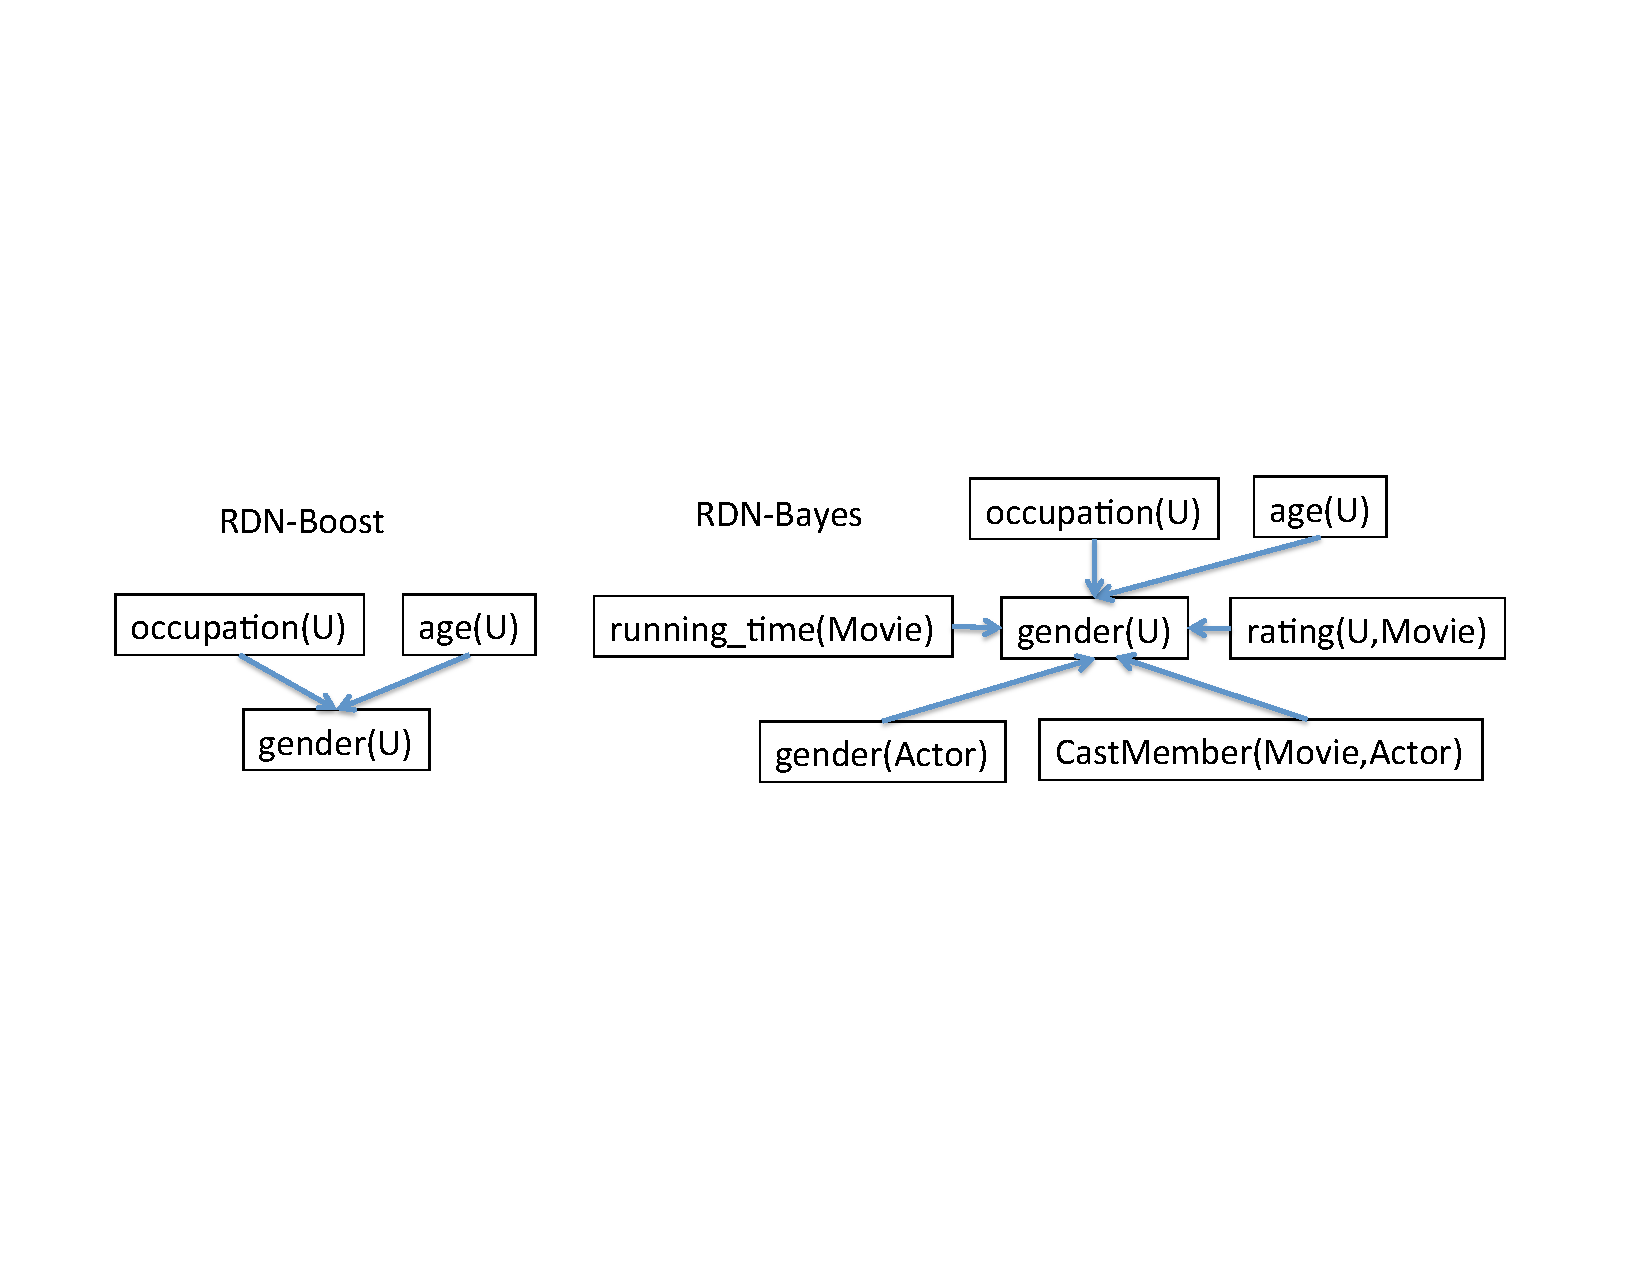
\includegraphics[width=1\textwidth]{figures/dn-structure}
%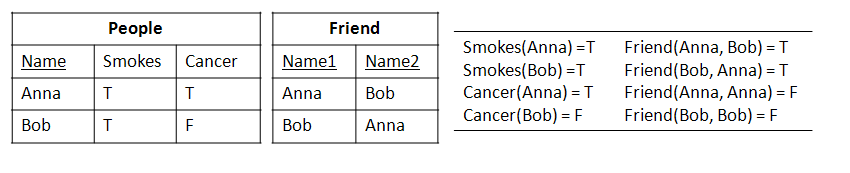
\includegraphics[width=1\textwidth]{database.png}
%}
\caption{The parents of the target $\it{gender}(\U)$ in the model discovered by RDN-Boost (top) and RDN-Bayes (bottom). \label{fig:dn-structure}}
\end{center}
\end{figure}


 
 
 
 
%% Table generated by Excel2LaTeX from sheet 'temp'
%\begin{table}[htbp]
%  \centering
%  \caption{Add caption}
%    \begin{tabular}{|r|r|r|r|r|r|}
%    \hline
%    dababase & \# of functor in MB & \# extra first order variable & CLL-diff & PR-diff & target node  \\
%    \hline
%    imdb  & 8/2   & 3/0   & 0.30  & 0.68  & u\_gender\_f  \\
%    \hline
%    uw    & 4/0   & 1/0   & 0.50  & 0.55  & student\_0  \\
%    \hline
%    hep   & 6/2   & 2/0   & 0.20  & 0.25  & sex\_0  \\
%    \hline
%    mondial & 11/0  & 1/0   & 0.58  & 0.30  & class\_0  \\
%    \hline
%    muta  & 5/0   & 1/0   & 0.56  & 0.22  & ind1\_0  \\
%    \hline
%    movielens & 2/1   & 1/0   & 0.26  & 0.26  & Gender\_M  \\
%    \hline
%    \end{tabular}%
%  \label{tab:addlabel}%
%\end{table}%
%

%; as the inventors of the boosting method put it, ``we sacrifice comprehensibility for better predictive performance'' \cite{Natarajan2012}. 
\section{Related Work}
Dependency networks were introduced in \cite{Heckerman2000} and relational dependency networks in \cite{Neville2007}. 
Heckerman {\em et al.} compare Bayesian, Markov and dependency networks for nonrelational data. 

\emph{Bayesian networks.} There are several proposals for defining directed relational template models, based on graphs with directed edges or rules in clausal format \cite{Kersting2007,Getoor2007c}. Defining the probability of a child node conditional on multiple instantiations of a parent set requires the addition of combining rules \cite{Kersting2007} or aggregation functions \cite{Getoor2007c}. 
%As described by \cite{Kersting2007}, aggregate functions can be added to a Parametrized Bayesian network by including functor nodes with aggregates. 
Combining rules such as the arithmetic mean~\cite{Natarajan2008} combine global parameters with a local scaling factor, as does our log-linear model. In terms of combining rules,  our model uses the {\em geometric mean} rather than the arithmetic mean.\footnote{The geometric mean of a list of numbers $x_{1},\ldots,x_{n}$ is $(\prod_{i} x_{i})^{1/n}$. The logarithm of the geometric mean is therefore $1/n \sum_{i} \ln x_{i}$. Thus geometric mean = exp(average (logs)).} To our knowledge, the geometric mean has not been used before as a combining rule for relational data.  
%Another difference with template Bayesian networks is that the geometric mean is applied to the entire Markov blanket of the target node, whereas usually a combining rule applies only to the parents of the target node. 

\emph{Markov Networks.} Markov Logic Networks (MLNs) provide a logical template language for undirected graphical models. 
Richardson and Domingos propose transforming a Bayesian network to a Markov Logic network using moralization, with log-conditional probabilities as weights \cite{Domingos2009}. 
This is also the standard BN-to-MLN transformation recommended by the Alchemy system \cite{bib:bayes-convert}. A discriminative model can be derived from any MLN \cite{Domingos2009}.  The structure transformation was used in previous work \cite{Schulte2012}, where MLN parameters were learned, not computed in closed-form from BN parameters. The Gibbs conditional probabilities derived from an MLN obtained from converting a Bayesian network are the same as those defined by our log-linear Formula~\ref{def:log-diff-freq-eq}, {\em if} counts replace proportions as feature functions \cite{Schulte2011}. There is no MLN whose discriminative model is equivalent to our log-linear equation with  proportions as feature functions.\footnote{Disclaimer: A preliminary version of this paper was presented at the StarAI 2012 workshop, with no archival proceedings. A previous version of this paper was accepted for publication in the ILP 2014 proceedings. We have elected to submit this work to the MLJ special issue instead of the ILP proceedings. We are indebted to StarAI and ILP reviewers and participants for helpful comments.}
 

\section{Conclusion and Future Work} 
\label{sec:conclusion}
Relational dependency networks offer important advantages for modelling relational data. We proposed a novel approach to learning dependency networks: first learn a Bayesian network, then perform a closed-form transformation of the Bayesian network to a dependency network. The key question is how to transform BN parameters to DN parameters. We introduced a new relational adapation of the standard BN log-linear equation for the probability of a target node conditional on an assigment of values to its Markov blanket. The new log-linear equation uses a sum of expected values of BN log-conditional probabilities, with respect to a random instantiation of first-order variables. This is equivalent to using feature instantiation proportions as feature functions. We compared our approach to state-of-the-art functional gradient boosting methods  on five benchmark datasets. Learning RDNs via BNs scales much better to large datasets than with boosting, and provides competitive accuracy in predictions.

Learning a collection of discriminative models and learning a Bayesian network are two very different approaches to constructing dependency networks, each with strengths and weaknesses. There are various options for hybrid approaches that combine the strengths of both. (1) Fast Bayesian network learning methods can be used to select features. Discriminative learning methods should work  faster restricted to the BN Markov blanket of a target node. (2) The Bayesian network can provide an initial dependency network structure. Gradient boosting can then be used to fine-tune a discriminative model of a child node given parent nodes, replacing a flat conditional probability table. In sum, learning relational dependency networks via Bayesian networks is a novel approach that offers promising advantages for  interpretability and scalability.

%\section*{Acknowledgements} 
%%This work was supported by Discovery Grants to Oliver Schulte from the Natural Science and Engineering Council of Canada. Zhensong Qian was supported by a grant from the China Scholarship Council. 
%A preliminary version of this paper was presented at the StarAI 2012 workshop. We are indebted to workshop reviewers and participants for helpful comments.

\section*{Appendix: Proof of Consistency Characterization} 

Claim: if there is a suitable edge, then there will be a grounding that makes for inconsistency.  Existence of suitable edge depends on population variables. Could make stronger claims too perhaps, they key thing is the different population variables. 


Let $\QC$ denote an assignment of values to all ground nodes other than the target nodes $\FG{\TT_{1}}$ and $ \FG{\TT_{2}}$. The log-linear equation~\ref{def:log-diff-freq-eq}, specifies the conditional distribution of each target node given $\QC$ and a value for the other target node. We keep the assignment $\QC$ fixed throughout, so for more compact notation, we abbreviate the conditional distributions as

$$\joint(\FG{{\TT_{1}}} = \TV_{1}| \FG{{\TT_{2}}} = \TV_{2}) \equiv P(\FG{{\TT_{1}}} = \TV_{1}|\FG{{\TT_{2}}} = \TV_{2},\QC)$$ 

and similarly for $P(\FG{{\TT_{1}}} = \TV_{1}|\FG{{\TT_{2}}} = \TV_{2},\QC)$.

On the assumption that the dependency network is consistent, there is a joint distribution over the target nodes conditional on the assignment that agrees with the conditional distribution:

$$\frac{\joint(\FG{{\TT_{1}}} = \TV_{1}, \FG{{\TT_{2}}} = \TV_{2})}{\joint(\FG{{\TT_{2}}} = \TV_{2})}= \joint(\FG{{\TT_{1}}} = \TV_{1}| \FG{{\TT_{2}})}$$
and also with the conditional $\joint(\FG{{\TT_{2}}} = \TV_{2}| \FG{{\TT_{1}}}=\TV_{1}).$

Lowd pointed out that 
this joint distribution satisfies the equations

\begin{equation}  \frac{\joint(\false,\false)}{\joint(\true,\false)} \cdot \frac{\joint(\true,\false)}{\joint(\true,\true)}= \frac{\joint(\false,\false)}{\joint(\true,\true)} = \frac{\joint(\false,\false)}{\joint(\false,\true)} \cdot \frac{\joint(\false,\true)}{\joint(\true,\true)} \label{eq:lowd-joint}
\end{equation}

Since the ratio of joint probabilities is the same as the ratio of conditional probabilities for the same conditioning event, consistency entails the following constraint on conditional probabilities via Equation~\eqref{eq:lowd-joint}:

\begin{equation}
\frac{\joint(\FG{{\TT_{2}}}=\false|\FG{{\TT_{1}}}=\false)}{\joint(\FG{{\TT_{2}}} = \true| \FG{{\TT_{1}}}=\false)} \cdot \frac{\joint(\FG{{\TT_{1}}}=\false|\FG{{\TT}_{2}}=\true)}{\joint(\FG{{\TT_{1}}} = \true| \FG{{\TT_{2}}}=\true)} =\frac{\joint(\FG{{\TT_{1}}}=\false|\FG{{\TT_{2}}}=\false)}{\joint(\FG{{\TT_{1}}} = \true| \FG{{\TT_{2}}}=\false)} \cdot \frac{\joint(\FG{{\TT_{2}}}=\false|\FG{{\TT_{1}}}=\true)}{\joint(\FG{{\TT_{2}}} = \true| \FG{{\TT_{1}}}=\true)} \label{eq:lowd-conditional}
\end{equation}
We refer to Equation~\ref{eq:lowd-conditional} as {\em Lowd's equation}. 
Satisfying Lowd's equations is both necessary and sufficient for a dependency network to be consistent.
The idea of our proof is to show that Lowd's equations are satisfied only if the relevant family counts for the target nodes are the same. According to the log-linear equation, each conditional probability is proportional to a product of BN parameters. The first step is to show that in Lowd's equation, all BN parameter terms cancel out except for those that are derived from the family that comprises $\FG{\TT_{1}}$ and their $\FG{\TT_{2}}$ and their common grounding. This may not hold in general, but can be proved provided that the edge $\TT_{1} \rightarrow \TT_{2}$ satisfies two conditions.

\begin{definition} \label{def:suitable}
An template edge $\TT_{1} \rightarrow \TT_{2}$ is \textbf{suitable} if

\begin{enumerate}
\item It is possible to find a grounding $\grounding$ for both parent and child, and an assignment $\QC$ to all other nodes, such that the relevant family count for the $\TT_{2}$ family differs for $\FG{\TT_{1}} = \grounding \TT_{1}$ 
and $\FG{\TT_{2}} = \grounding \TT_{2}$.
\item the parent and child have no common edge.
\end{enumerate}
\end{definition}

The first condition says that it is possible to ground the template edge in such a way as to obtain different relevant family counts, which is the key condition for inconsistency. This is possible if and only if some parent and child contain a different set of population variables. (Otherwise the relevant family counts are always 1.) The second condition is useful because it means that in the log-linear equations for the ground parent and ground child, the only terms that involve both of them are groundings of the family of $\TT_{2}$. The next lemma asserts the existence of a suitable edge. 

\begin{lemma}
Suppose that the template BN contains an edge such that the parent and child contain a different set of population variables. Then the template BN contains a suitable edge.
\end{lemma}
\begin{proof}
Suppose that there is an edge satisfying the population variable condition. Suppose that the parent and child share a common child. Since the edge satisfies the condition, the set of population variables in the common child differs from at least one of  $\TT_{1}, \TT_{2}$. Therefore there is another edge from one of  $\TT_{1} \rightarrow \TT_{2}$ as parent to a new child that satisfies the population variable condition. If this edge is not suitable, there must be another shared child. Repeating this argument, we eventually arrive at an edge satisfying the population variable condition  where the child node is a sink node without children. This edge is suitable.
\end{proof}
\marginpar{perhaps insert figure of graph and groundings}

Consider a suitable template edge $\TT_{1} \rightarrow \TT_{2}$ that produces a bidirected edge $\FG{\TT_{1}} \leftrightarrow \FG{\TT_{2}}$. For simplicity we assume that $\TT_{1}$ and $\TT_{2}$ are binary variables with domain $\{\true,\false\}$. \marginpar{need some comment} Let $\Pa{\TT_{2}}$ be the parents of $\TT_{2}$ other than $\TT_{1}$. Since the template edge is not redundant, there is a parent value setting $\Pa{\TT_{2}} = \parents$ such that $\TT_{1}$ and $\TT_{2}$ are conditionally dependent given $\Pa{\TT_{2}} = \parents$. This implies that the conditional distribution of $\TT_{1}$ is different for each of the two possible values of $\TT_{2}$. In terms of the template Bayesian network parameters, this implies that

\begin{equation} \label{eq:dependence}
\frac{\cprob{\TT_{2} = \false}{\TT_{1} = \false,\parents}}{\cprob{\TT_{2} = \true}{\TT_{1} = \false,\parents}} \neq \frac{\cprob{\TT_{2} = \false}{\TT_{1} = \true,\parents}}{\cprob{\TT_{2} = \true}{\TT_{1} = \true,\parents}}.
\end{equation}

Since the edge $\TT_{1} \rightarrow \TT_{2}$ is suitable, it is possible to find ground \textbf{target nodes} $\FG{\TT_{1}}$, $\FG{\TT_{2}}$, and an assignment $\QC$ to all other nodes, such that the relevant family counts for the $\TT_{2}$ family differs between the target nodes. Moreover without loss of generality we can assume that  the only $\QC$ groundings for the parents of $\FG{\TT_{2}}$ agree with the values $\parents$. We refer to such a choice of input variables $\QC$ as \textbf{suitable}.


\begin{lemma} \label{lemma:decompose-cond}
Suppose that $\TT_{1} \rightarrow \TT_{2}$ is a suitable edge with suitable groundings $\FG{\TT_{1}}$,$\FG{\TT_{2}}$,$\QC$. The only instantiated groundings for the parents of $\FG{\TT_{2}}$ agree with the values $\parents$. Then for any target node values $\TV_{1}$ and $\TV_{2}$, we can write the conditional probabilities as follows:

\begin{equation}
\Gprob{\FG{{\TT_{2}}} = \TV_{2}} {\FG{\TT_{1}} = \TV_{1},\QC} \propto \cprob{\TT_{2} = \TV_{2}}{\TT_{1} = \TV_{1},\parents}^{(N/N_{2}+M_{\TT_2=\TV_{2}}/N_{2})} \cdot \pi_{\TT_2=\TV_{2}} \label{eq:decompose-t2}
\end{equation}
where $M_{\TT_2=\TV_{2}}$ and $\pi_{\TT_2=\TV_{2}}$ depend only on $\TV_{2}$ and not on $\TV_{1}$ and
\begin{equation}
\Gprob{\FG{{\TT_{1}}} = \TV_{1}} {\FG{\TT_{2}} = \TV_{2},\QC} \propto \cprob{\TT_{2} = \TV_{2}}{\TT_{1} = \TV_{1},\parents}^{(N/N_{1}+M_{\TT_1=\TV_{1}}/N_{1})} \cdot \pi_{\TT_1=\TV_{1}} \label{eq:decompose-t1}
\end{equation} 
where $M_{\TT_1=\TV_{1}}$ and $\pi_{\TT_1=\TV_{1}}$ depend only on $\TV_{1}$ and not on $\TV_{2}$.
\end{lemma}

\begin{proof}
We start with target node $\FG{\TT_{2}}$. (1) The log-linear equation~\ref{def:log-diff-freq-eq} contains a term for the children of $\FG{\TT_{2}}$. Since $\TT_{1}$ and $\TT_{2}$ share no children, the corresponding conditional probabilities do not depend on the value of $\FG{\TT_{1}}$, but only on $\QC$ and $\TT_{2}$. Thus the product of the BN parameters can be denoted as $\pi_{\TT_2=\TV_{2}}$. (2) The only other term in the log-linear equation is for the family of $\FG{\TT_{2}}$. Since $\QC$ is suitable, the only instantiated groundings for the parents of $\FG{\TT_{2}}$ agree with the values $\parents$. These groundings can be divided into those that agree with $\FG{\TT_{1}}$ and those that do not. (3) The log-linear terms for the latter do not depend on the value $\TV_{1}$ of $\FG{\TT_{1}}$,  hence their number can be written as $M_{\TT_2=\TV_{2}}$. (4) For groundings that are consistent with both  $\FG{\TT_{1}}$ and $\FG{\TT_{2}}$, their number does not depend on the values of $\FG{\TT_{1}}$ or $\FG{\TT_{2}}$. It depends only on $\QC$. Let this number be $N$. 

Now consider target node $\FG{\TT_{1}}$. (1) The log-linear equation~\ref{def:log-diff-freq-eq} contains a term for the family of $\FG{\TT_{1}}$. Since $\TT_{1}$ is a parent of $\TT_{2}$, the acyclicity of the template BN entails that $\TT_{2}$ is not a parent of $\TT_{1}$. Therefore  the conditional probabilities for the family of $\FG{\TT_{1}}$ do not depend on the value of $\FG{\TT_{2}}$, but only on $\QC$ and $\TT_{1}$. (2) The log-linear equation~\ref{def:log-diff-freq-eq} also contains a term for the children of $\TT_{1}$ other than $\TT_{2}$. Since the edge $\TT_{1} \rightarrow \TT_{2}$ is suitable, the two nodes do not share a child, so these terms also do not depend on the value of $\FG{\TT_{2}}$. Thus collectively, the product of the terms (1) and (2) can be written as $\pi_{\TT_1=\TV_{1}} $. The remaining terms are groundings for $\FG{\TT_{1}}$ and the family of $\TT_{2}$. These groundings can be divided into those that agree with $\FG{\TT_{2}}$ and those that do not. (3) The log-linear terms for the latter do not depend on the value $\TV_{2}$ of $\FG{\TT_{2}}$,  hence their number can be written as $M_{\TT_1=\TV_{1}}$. (4) The number of groundings that are consistent with both  $\FG{\TT_{1}}$ and $\FG{\TT_{2}}$ is denoted by $N$ as above.
\end{proof}

\marginpar{discuss if conditions can be relaxed}
\begin{lemma}
Suppose that conditions~\eqref{eq:decompose-t2} and~\eqref{eq:decompose-t1} of Lemma~\ref{lemma:decompose-cond} hold. Then Lowd's Equation~\eqref{eq:lowd-conditional} holds if and only if $N_{1} = N_{2}$. 
\end{lemma}

\begin{proof}
Observe that in Equation~\eqref{eq:lowd-conditional}, each term on the left has a corresponding term with the same value for the target node assignment and the opposing conditioning assignment. For instance, the term $\joint(\FG{{\TT_{2}}}=\false|\FG{{\TT_{1}}}=\false)$ on the left is matched with the term $\joint(\FG{{\TT_{2}}}=\false|\FG{{\TT_{1}}}=\true)$ on the right. This means that the products in the log-linear expression are the same on both sides of the equation except for those factors that depend on {\em both} $\TV_{1}$ and $\TV_{2}$. Continuing the example, the factors $$\cprob{\TT_{2} = \false}{\TT_{1} = \false,\parents}^{(M_{\false}/N_{2})} \cdot \pi_{\TT_2=\TV_{2}}$$ on the left equal the factors $$\cprob{\TT_{2} = \false}{\TT_{1} = \true,\parents}^{(M_{\TT_1=\TV_{1}}/N_{2})}\cdot \pi_{\TT_2=\TV_{2}}$$ on the right side of the equation. They therefore cancel out, leaving only the term $$\cprob{\TT_{2} = \false}{\TT_{1} = \false,\parents}^{N/N_{2}}$$ on the left and the term $$\cprob{\TT_{2} = \false}{\TT_{1} = \false,\parents}^{N/N_{2}}$$ on the right. Lowd's equation can therefore be reduced to an equivalent constraint with only such BN parameter terms. For further compactness we abbreviate such terms as follows

$$\cprob{\TV_{2}}{\TV_{1}} \equiv \cprob{\TT_{2} = \TV_{2}}{\TT_{1} = \TV_{1},\parents}.$$ With this abbreviation, the conditions of Lemma~\ref{lemma:decompose-cond} entail that Lowd's equation~\ref{eq:lowd-conditional} reduces to the equivalent expressions.


\begin{eqnarray}
\frac{\cprob{\false}{\false}^{N/N_{2}}}{\cprob{\true}{\false}^{N/N_{2}} }  \cdot \frac{\cprob{\true}{\false}^{N/N_{1}} }{\cprob{\true}{\true}^{N/N_{1}} }  & = & \frac{\cprob{\false}{\false}^{N/N_{1}} }{\cprob{\false}{\true}^{N/N_{1}} }  \cdot \frac{\cprob{\false}{\true}^{N/N_{2}} }{\cprob{\true}{\true}^{N/N_{2}} } \\
(\frac{\cprob{\false}{\false}}{\cprob{\true}{\false} })^{\left(N/N_{2}-N/N_{1}\right)}   & = &  (\frac{\cprob{\false}{\true} }{\cprob{\true}{\true}})^{\left(N/N_{2}-N/N_{1}\right)} \label{eq:transform-ratio}
\end{eqnarray}

By the nonredundancy  assumption~\eqref{eq:dependence} on the BN parameters, we have

$$\frac{\cprob{\false}{\false}}{\cprob{\true}{\false} }   \neq  \frac{\cprob{\false}{\true} }{\cprob{\true}{\true}}$$

so Equation~\ref{eq:transform-ratio} implies that 

$$N_{1} = N_{2}, $$ which establishes the lemma. 

\end{proof}

Equation~\eqref{eq:lowd-conditional} provides a constraint on the conditional distributions defined by the log-linear equation~\eqref{def:log-diff-freq-eq}. We show that given the choice of the grounding $\QC$, this equation is satisfied if and only if the relevant family counts of $\FG{TT_{1}}$ and $\FG{\TT_{2}}$ in the target family are the same, i.e. $N_{1} = N_{2}$. 


\begin{proof}
Cleaner proof: 1) assume dependence assumption throughout. 2) if some edge does not have the same population variables, then there is a grounding that leads to inconsistency. 

2a) Construct suitable edge.
2b) Choose joint grounding of suitable edge, and lambda* s.t. the ground family of the suitable edge has only two possible states, where the co-parent induces dependence between parent and child, and the child and parent have only the two possible values that are dependent.
2c) Assume a joint probability between the two ground nodes given lambda*. Use Lowd's equation to show the equivalence of two different ways of decomposing that. 
2d) Divide families into the target family and other families. Show a set of paired equations, one for parent*, one for child*. s.t. we can focus on target family only.
2e) Divide the groundings of target family into those that satisfy master grounding and those that don't. Show that the others cancel out in Lowd's equation, using pairs of equations.
2f) Show that for the grounding that satisfies the master family, the number of groundings is a constant independent of the values of parent* and child*. Rewrite Lowd's equation using this fact.
2g) Transform the rewritten Lowd equation in terms of the dependence on T1*. Conclude that the number of groundings must be the same, contrary to assumption.

($\Leftarrow$) If the relevant family counts are constant, we can define an MLN that matches the dependency network.
($\Rightarrow$) Our strategy is to start with a suitable edge in the Bayesian network template. For the suitable edge, we construct a grounding of parent, child and an assignment of values to all other ground nodes. For such an assignment, the log-linear equations define a conditional distribution of the ground parent node given a value for the ground child node, and conversely a conditional distribution of the ground child node, given a value for the ground parent node. We show that, conditional on the joint assignment, there is no joint distribution of the ground parent and child node, that is consistent with the two conditional distributions. 

A suitable edge $\TT_{1} \rightarrow \TT_{2}$ satisfies the following two conditions: (1) it is possible to find a grounding $\grounding$ for both parent and child, and an assignment $\QC$ to other all other nodes, such that the relevant family count for the $\TT_{2}$ family differs for $\FG{\TT_{1}} = \grounding \TT_{1}$ 
and $\FG{\TT_{2}} = \grounding \TT_{2}$, and (2) the parent and child have no common edge. To argue that such an edge must exist in the template BN, we observe that condition (1) is satisfied if and only if the parent and child do not contain the same set of population variables. If there is no edge satisfying condition (1), then all relevant family counts are guaranteed to be the same, and the dependency network is consistent. Otherwise suppose that there is an edge satisfying condition (1). Suppose that the parent and child share a common child. Since the edge satisfies condition (1), parent and child do not contain the same set of population variables. Therefore the set of population variables in the common child differs from at least one of  $\TT_{1}, \TT_{2}$. Therefore there is another edge from one of  $\TT_{1} \rightarrow \TT_{2}$ as parent to a new child that satisfies condition (1). If this edge is not suitable, there must be another shared child. Repeating this argument, we eventually arrive at an edge satisfying condition (1) where the child node is a sink node without children. This edge is suitable.

Consider a suitable template edge $\TT_{1} \rightarrow \TT_{2}$ that produces a bidirected edge $\FG{\TT_{1}} \leftrightarrow \FG{\TT_{2}}$. For simplicity we assume that $\TT_{1}$ and $\TT_{2}$ are binary variables with domain $\{\true,\false\}$. \marginpar{need some comment} Let $\Pa{\TT_{2}}$ be the parents of $\TT_{2}$ other than $\TT_{1}$. Since the template edge is not redundant, there is a parent value setting $\Pa{\TT_{2}} = \parents$ such that $\TT_{1}$ and $\TT_{2}$ are conditionally dependent given $\Pa{\TT_{2}} = \parents$. This implies that the conditional distribution of $\TT_{1}$ is different for each of the two possible values of $\TT_{2}$. In terms of the template Bayesian network parameters, this implies that

\begin{equation} \label{eq:dependence}
\frac{\cprob{\TT_{2} = \false}{\TT_{1} = \false,\parents}}{\cprob{\TT_{2} = \true}{\TT_{1} = \false,\parents}} \neq \frac{\cprob{\TT_{2} = \false}{\TT_{1} = \true,\parents}}{\cprob{\TT_{2} = \true}{\TT_{1} = \true,\parents}}.
\end{equation}

To simplify the notation in our proof, we introduce the following abbreviation:

$$\psi_{\TV_{2}|\TV_{1}} \equiv \cprob{\TT_{2} = \TV_{2}}{\TT_{1} = \TV_{1},\parents}.$$



Let $\QC$ denote an assignment of values to all ground nodes other than $\FG{\TT_{1}}$ and $ \FG{\TT_{2}}$. \marginpar{consider Daniel Lowd's minus notation for this} There is a unique family in the template BN that contains the template edge $\TT_{1} \rightarrow \TT_{2}$. Let $N_{2}$ be the sum of all relevant family counts for the family $(\Appendterm{\TT_{2}} {\Pa{\TT_{2}}})$ given the grounding that defines $ \FG{\TT_{2}}$. Similarly, let $N_{1}$ be the sum of all relevant family counts for the same family $(\Appendterm{\TT_{2}} {\Pa{\TT_{2}}})$, given the grounding that defines $ \FG{\TT_{1}}$. From the log-linear equation~\ref{def:log-diff-freq-eq}, the conditional probability of $\FG{\TT_{2}}= \TV_{2}$ given $\QC, \FG{\TT_{1}} = \TV_{1}$ is proporational to a product of conditional probability terms raised to the power of $1/N_{2}$, times a product of similar conditional probability terms for the families of children of $\FG{\TT_{2}}$. We may therefore write 

$$\Gprob{\FG{{\TT_{2}}} = \TV_{2}} {\QC,\FG{\TT_{1}} = \TV_{1}} \propto \cprob{\TT_{2} = \TV_{2}}{\TT_{1} = \TV_{1},\parents}^{1/N_{2}} \cdot \sigma_{\TV_{2}}$$ where 
$\sigma_{\TV_{2}}$ is a product of smoothed conditional probability values. Similarly, we may write $$\Gprob{\FG{{\TT_{1}}} = \TV_{1}} {\QC,\FG{\TT_{2}} = \TV_{2}} \propto \cprob{\TT_{2} = \TV_{2}}{\TT_{1} = \TV_{1},\parents}^{1/N_{1}} \cdot \sigma_{\TV_{1}}$$. \marginpar{may have to make product depend on both t1 and t2} 

On the assumption that the dependency network is consistent, there is a joint distribution 

$$\joint(\FG{{\TT_{1}}} = \TV_{1}, \FG{{\TT_{2}}} = \TV_{2}) \equiv P(\FG{{\TT_{1}}} = \TV_{1}, \FG{{\TT_{2}}} = \TV_{2}|\QC).$$

This joint distribution satisfies the equations

\begin{equation*}
\frac{\joint(\false,\false)}{\joint(\true,\true)} = \frac{\joint(\false,\false)}{\joint(\false,\true)} \cdot \frac{\joint(\false,\true)}{\joint(\true,\true)}
\end{equation*}

and 

\begin{equation*}
\frac{\joint(\false,\false)}{\joint(\true,\true)} = \frac{\joint(\false,\false)}{\joint(\true,\false)} \cdot \frac{\joint(\true,\false)}{\joint(\true,\true)}
\end{equation*}

Therefore we have the equations

\begin{eqnarray}
\frac{\joint(\false,\false)}{\joint(\false,\true)} \cdot \frac{\joint(\false,\true)}{\joint(\true,\true)}&=&\frac{\joint(\false,\false)}{\joint(\true,\false)} \cdot \frac{\joint(\true,\false)}{\joint(\true,\true)} \\ \label{eq:joint}
\frac{\joint(\FG{{\TT_{2}}}=\false|\FG{{\TT_{1}}}=\false)}{\joint(\FG{{\TT_{2}}} = \true| \FG{{\TT_{1}}}=\false)} \cdot \frac{\joint(\FG{{\TT_{1}}}=\false|\FG{{\TT}_{2}}=\true)}{\joint(\FG{{\TT_{1}}} = \true| \FG{{\TT_{2}}}=\true)}&=&\frac{\joint(\FG{{\TT_{1}}}=\false|\FG{{\TT_{2}}}=\false)}{\joint(\FG{{\TT_{1}}} = \true| \FG{{\TT_{2}}}=\false)} \cdot \frac{\joint(\FG{{\TT_{2}}}=\false|\FG{{\TT_{1}}}=\true)}{\joint(\FG{{\TT_{2}}} = \true| \FG{{\TT_{1}}}=\true)} \label{eq:lowd-conditional}
\end{eqnarray}

Equation~\eqref{eq:lowd-conditional} provides a constraint on the conditional distributions defined by the log-linear equation~\eqref{def:log-diff-freq-eq}. We show that given the choice of the grounding $\QC$, this equation is satisfied if and only if the relevant family counts of $\FG{TT_{1}}$ and $\FG{\TT_{2}}$ in the target family are the same, i.e. $N_{1} = N_{2}$. The log-linear equation for target $\FG{\TT_{1}}$ sums over all BN families containing $\FG{\TT_{1}}$. These families can be divided into those that contain only the template node $\TT_{1}$ and those that contain both $\TT_{1}$ and $\TT_{2}$. We show that we need take into account only families that contain both. Consider a family that instantiates only the template node $\TT_{1}$ and the corresponding term
$$
\qquad \left[ \ln \cprob{\UT = \UV}{\Pa{\UT} = \Prange{\UT}} \right]  \cdot   \Relfreq{\Appendterm{\grounding;\UT  = \UV} {\Pa{\UT} = \Prange{\UT}}} {\QC,\FG{\TT_{1}} = \TV_{1},\FG{\TT_{2}} = \true}
$$
where we arbitrarily set $\FG{\TT_{2}} = \true$ for the sake of concreteness. Since $\FG{\TT_{2}}$ does not appear in any instance of the family, the family frequency is independent of $\FG{\TT_{2}}$. In symbols, we have
%
$$
 \Relfreq{\Appendterm{\grounding;\UT  = \UV} {\Pa{\UT} = \Prange{\UT}}} {\QC,\FG{\TT_{1}} = \TV_{1},\FG{\TT_{2}} = \true} = \Relfreq{\Appendterm{\grounding;\UT  = \UV} {\Pa{\UT} = \Prange{\UT}}} {\QC,\FG{\TT_{1}} = \TV_{1},\FG{\TT_{2}} = \false}.
$$
Now notice that for every conditional probability of the form $$\joint(\FG{\TT_{1}}=\TV_{1}|\FG{\TT_{2}}=\false)$$ on one side of the equation~\ref{eq:lowd-conditional}, there is a corresponding conditonal probability term of the form $$\joint(\FG{\TT_{1}}=\TV_{1}|\FG{\TT_{2}}=\true)$$ on the other side. Therefore the log-linear terms that involve families with $\TT_{1}$ but not $\TT_{2}$ cancel out. The same argument can be made for families that involve $\TT_{2}$ but not $\TT_{1}$. Therefore we need consider only terms for families that contain both $\TT_{1}$ and $\TT_{2}$. Since by choice of $\TT_{1}$ and $\TT_{2}$, the two nodes don't share common children, the only family that contains both $\TT_{1}$ and $\TT_{2}$ is the one with $\TT_{2}$ as its child. We refer to this family as the {\em target family}. 

The groundings of this family for target $\FG{\TT_{1}}$ can be divided into those that are consistent with $\FG{\TT_{2}}$ and those that are not. If a grounding is not consistent with $\FG{\TT_{2}}$, then the corresponding family instance configuration is independent of the value assigned to $\FG{\TT_{2}}$. In symbols, we have

$\Relcount{\Appendterm{\grounding_{1};\TT_{2}  = \TV_{2}} {\Pa{\TT_{2}} = \parents}} {\QC,\FG{\TT_{1}} = \TV_{1},\FG{\TT_{2}} = \true} = \Relcount{\Appendterm{\grounding_{1};\TT_{2}  = \TV_{2}} {\Pa{\TT_{2}} = \parents}} {\QC,\FG{\TT_{1}} = \TV_{1},\FG{\TT_{2}} = \false}$

where the number of groundings excludes groundings consistent with $\FG{\TT_{2}}$. \marginpar{We need notation for this}. The same argument works for $\FG{\TT_{2}}$. As with the division of families, this implies that terms on the left cancel terms on the right, such that the only groundings that are counted are those that are consistent with both  $\FG{\TT_{1}}$ and $\FG{\TT_{2}}$ (call this master grounding $\grounding$, need to choose initial grounding so that this exists). The number of such groundings for a given target family configuration does not depend on the value of $\FG{\TT_{1}}$ or $\FG{\TT_{2}}$, only on $\QC$ via the constants that appear in $\grounding$. Let this constant number be $N$. \marginpar{focus attention only on the parent state that makes $\TT_{1}$ dependent with $\TT_{2}$}. Then using the abbreviation above, Equation~\eqref{eq:lowd-conditional} is equivalent to

\begin{eqnarray}
\frac{\cprob{\false}{\false}^{N/N_{2}}}{\cprob{\true}{\false}^{N/N_{2}} }  \cdot \frac{\cprob{\true}{\false}^{N/N_{1}} }{\cprob{\true}{\true}^{N/N_{1}} }  & = & \frac{\cprob{\false}{\false}^{N/N_{1}} }{\cprob{\false}{\true}^{N/N_{1}} }  \cdot \frac{\cprob{\false}{\true}^{N/N_{2}} }{\cprob{\true}{\true}^{N/N_{2}} } \\
(\frac{\cprob{\false}{\false}}{\cprob{\true}{\false} })^{\left(N/N_{2}-N/N_{1}\right)}   & = &  (\frac{\cprob{\false}{\true} }{\cprob{\true}{\true}})^{\left(N/N_{2}-N/N_{1}\right)} \label{eq:transform-ratio}\\
(\frac{\cprob{\false}{\false}}{\cprob{\true}{\false} })   & = &  (\frac{\cprob{\false}{\true} }{\cprob{\true}{\true}})
\end{eqnarray}

Since by the dependence assumption on the Bayes net parameters, we have

$$(\frac{\cprob{\false}{\false}}{\cprob{\true}{\false} })   \neq  (\frac{\cprob{\false}{\true} }{\cprob{\true}{\true}})$$

Equation~\ref{eq:transform-ratio} implies that 

$$N_{1} = N_{2}. $$ Since this contradicts the choice of the grounding, it follows that Equation~\ref{eq:joint} does not hold, so the dependency network is not consistent for the grounding $\QC$.
 \end{proof}



\bibliographystyle{plain}
\bibliography{master}
\end{document}
